\documentclass[11pt,oneside]{report}

% Motor: lualatex (Unicode nativo, sin necesidad de inputenc/fontenc).
\usepackage{fontspec}
% Respaldo de glifos: ver FONT_SETUP en build_reference_manual.py.
\directlua{
  luaotfload.add_fallback("solidumserif", {"DejaVuSerif:mode=node;", "DejaVuSans:mode=node;", "SegoeUISymbol:mode=node;", "SegoeUIEmoji:mode=node;"})
  luaotfload.add_fallback("solidummono", {"DejaVuSansMono:mode=node;", "DejaVuSans:mode=node;", "SegoeUISymbol:mode=node;", "SegoeUIEmoji:mode=node;"})
}
\setmainfont{Latin Modern Roman}[RawFeature={fallback=solidumserif}]
\setsansfont{Latin Modern Sans}[RawFeature={fallback=solidumserif}]
\setmonofont{Latin Modern Mono}[RawFeature={fallback=solidummono}]
\usepackage[protrusion=true,expansion=true]{microtype}
\usepackage{graphicx}
\usepackage{float}
\usepackage[spanish,es-tabla,es-nodecimaldot]{babel}
\usepackage[paperwidth=19.2cm, paperheight=25.6cm, hmargin=1.3cm, top=2.1cm, bottom=1.7cm, headheight=15pt, headsep=0.45cm, footskip=0.75cm]{geometry}
\usepackage{listings}
\usepackage{xcolor}
\usepackage{hyperref}
\usepackage{titlesec}
\usepackage{amsmath}
\usepackage{amssymb}
\usepackage{amsfonts}
% Corchetes dobles \llbracket [[u]] \rrbracket: notación del salto de
% desplazamientos en discontinuidades embebidas y materiales cohesivos
% (ADR 0010). No están en amssymb.
\usepackage{stmaryrd}
\usepackage{booktabs}
\usepackage{tabularx}
\usepackage{array}
\usepackage{ragged2e}
\usepackage{fancyhdr}
\usepackage{microtype}
\usepackage[most]{tcolorbox}

\newcolumntype{Y}{>{\RaggedRight\arraybackslash\footnotesize}X}

\definecolor{yamlkey}{RGB}{0, 102, 204}
\definecolor{yamlval}{RGB}{204, 0, 0}
\definecolor{yamlcomment}{RGB}{120, 120, 120}
\definecolor{bglight}{RGB}{245, 245, 245}
\definecolor{darkgray}{RGB}{50, 50, 50}
\definecolor{notebackground}{RGB}{240, 248, 255}
\definecolor{noteborder}{RGB}{0, 102, 204}
\definecolor{warnbackground}{RGB}{255, 245, 230}
\definecolor{warnborder}{RGB}{204, 102, 0}

% Cuadro de informacion: usado por los bloques `callout Nota`.
\newtcolorbox{infobox}[1]{
  enhanced,
  colback=notebackground, colframe=noteborder, colbacktitle=notebackground,
  coltitle=noteborder, fonttitle=\bfseries,
  title=#1, attach boxed title to top left={yshift=-2mm, xshift=4mm},
  boxed title style={colback=white, colframe=white, sharp corners},
  boxrule=0.4pt, arc=2pt,
  left=4mm, right=4mm, top=2mm, bottom=2mm,
  before skip=8pt, after skip=8pt,
}

% Cuadro de advertencia: usado por los bloques `callout Advertencia`.
% Comparte el comando ``\begin{infobox}{Advertencia}'' del conversor; los
% bloques marcados con titulo "Advertencia" reciben el color naranja via
% redefinicion local de las claves de color (ver macro \warnbox abajo).
\newtcolorbox{warnbox}[1]{
  enhanced,
  colback=warnbackground, colframe=warnborder, colbacktitle=warnbackground,
  coltitle=warnborder, fonttitle=\bfseries,
  title=#1, attach boxed title to top left={yshift=-2mm, xshift=4mm},
  boxed title style={colback=white, colframe=white, sharp corners},
  boxrule=0.4pt, arc=2pt,
  left=4mm, right=4mm, top=2mm, bottom=2mm,
  before skip=8pt, after skip=8pt,
}

\hypersetup{
    colorlinks=true,
    linkcolor=yamlkey,
    urlcolor=yamlkey,
    pdftitle={Manual de Ejemplos - Solidum FEM},
    pdfauthor={Jaime Retama Velasco}
}

\titleformat{\chapter}[display]
  {\normalfont\huge\bfseries\color{yamlkey}}{\chaptertitlename\ \thechapter}{20pt}{\Huge}
\titleformat{\section}{\Large\bfseries\color{darkgray}}{\thesection}{1em}{}
\titleformat{\subsection}{\large\bfseries\color{darkgray}}{\thesubsection}{1em}{}
\titleformat{\subsubsection}{\normalsize\bfseries\color{darkgray}}{\thesubsubsection}{1em}{}

\renewcommand{\chaptermark}[1]{\markboth{Cap.\ \thechapter\ ---\ #1}{}}

\pagestyle{fancy}
\fancyhf{}
\fancyhead[L]{\textbf{\color{darkgray}Solidum FEM --- Ejemplos}}
\fancyhead[R]{\color{darkgray}\nouppercase{\leftmark}}
\fancyfoot[C]{\thepage}
\fancyfoot[R]{\footnotesize\color{darkgray}FF-ME}
\renewcommand{\headrulewidth}{0.4pt}
\renewcommand{\footrulewidth}{0.4pt}

\lstdefinelanguage{yaml}{
  keywords={nodes, materials, elements, mesh, mesh_material, mesh_thickness, mesh_quadrature, mesh_physical_groups, quadrature, boundary_conditions, boundary_conditions_by_node, boundary_conditions_by_coord, boundary_conditions_by_group, point_loads, point_loads_by_node, point_loads_by_coord, point_loads_by_group, body_force, gravity, density, linear_constraints, slave, masters, coefficients, g, dof, node, solver, output, file_name, pre_process, export, results, text_export, frequency, nodal_results, element_results, format, id, type, coords, ref_vector, A, I, Iy, Iz, J, As, E, nu, sigma_y, H, hypothesis, ux, uy, uz, rx, ry, rz, tol, coord, val, num_steps, max_iter, adaptive, tol_iter, max_lambda, initial_dl, initial_dlambda, initial_tau,max_steps, material, thickness, kappa_0, alpha, cohesion, phi_deg, psi_deg, variant, n_modes, sigma, which, tolerance, lumping, t_end, dt, beta, gamma, rayleigh, alpha_rayleigh, beta_rayleigh, xi1, omega1, xi2, omega2, u0, u0_dot, F_func, freeze_tangent_after_iter, convergence, rtol_force, rtol_disp, atol_force_factor, atol_disp_factor, caption, linear_algebra, min_delta_lambda},
  keywordstyle=\color{yamlkey}\bfseries,
  ndkeywords={true, false, null, all, all_steps, last_step, plane_stress, plane_strain, plane_strain_matched, outer_cone, inner_cone, consistent, lumped, LinearSolver, NonlinearSolver, ArcLengthSolver, ModalSolver, NewmarkSolver, NewtonNewmarkSolver, Elastic1D, Elastic2D, Elastoplastic1D, VonMises2D, IsotropicDamage1D, IsotropicDamage2D, DruckerPrager2D, CableMaterial1D, Truss2D, Truss2DCorot, Truss3D, Truss3DCorot, Cable2DCorot, Cable3DCorot, Frame2DEuler, Frame2DTimoshenko, Frame2DEulerCorot, Frame3D, Quad4, Quad8, Quad9, Tri3, Tri6},
  ndkeywordstyle=\color{yamlval}\bfseries,
  identifierstyle=\color{black},
  sensitive=false,
  comment=[l]{\#},
  commentstyle=\color{yamlcomment}\ttfamily,
  stringstyle=\color{yamlval}\ttfamily,
  morestring=[b]',
  morestring=[b]"
}

\lstset{
  basicstyle=\ttfamily\footnotesize,
  backgroundcolor=\color{bglight},
  frame=single,
  rulecolor=\color{lightgray},
  breaklines=true,
  showstringspaces=false,
  extendedchars=true,
  captionpos=b,
  literate={§}{{§}}1 {ª}{{ª}}1 {µ}{{µ}}1 {¹}{{¹}}1 {º}{{º}}1 {½}{{½}}1 {¿}{{¿}}1 {ê}{{ê}}1 {û}{{û}}1 {ć}{{ć}}1 {Γ}{{Γ}}1 {Σ}{{Σ}}1 {Φ}{{Φ}}1 {ζ}{{ζ}}1 {η}{{η}}1 {ξ}{{ξ}}1 {ψ}{{ψ}}1 {ᵀ}{{ᵀ}}1 {Ṫ}{{Ṫ}}1 {‖}{{‖}}1 {…}{{…}}1 {⁴}{{⁴}}1 {⁶}{{⁶}}1 {⁺}{{⁺}}1 {⁻}{{⁻}}1 {₀}{{₀}}1 {₁}{{₁}}1 {₂}{{₂}}1 {₃}{{₃}}1 {₆}{{₆}}1 {ₓ}{{ₓ}}1 {ℓ}{{ℓ}}1 {ℝ}{{ℝ}}1 {↔}{{↔}}1 {∂}{{∂}}1 {∇}{{∇}}1 {∈}{{∈}}1 {∉}{{∉}}1 {−}{{−}}1 {√}{{√}}1 {∞}{{∞}}1 {∫}{{∫}}1 {≈}{{≈}}1 {≡}{{≡}}1 {≪}{{≪}}1 {≲}{{≲}}1 {≳}{{≳}}1 {⊗}{{⊗}}1 {⟨}{{⟨}}1 {⟩}{{⟩}}1
           {á}{{\'a}}1 {é}{{\'e}}1 {í}{{\'i}}1 {ó}{{\'o}}1 {ú}{{\'u}}1
           {Á}{{\'A}}1 {É}{{\'E}}1 {Í}{{\'I}}1 {Ó}{{\'O}}1 {Ú}{{\'U}}1
           {ñ}{{\~n}}1 {Ñ}{{\~N}}1 {ü}{{\"u}}1 {Ü}{{\"U}}1
           {ε}{{$\varepsilon$}}1 {σ}{{$\sigma$}}1 {α}{{$\alpha$}}1
           {β}{{$\beta$}}1 {γ}{{$\gamma$}}1 {δ}{{$\delta$}}1
           {θ}{{$\theta$}}1 {κ}{{$\kappa$}}1 {λ}{{$\lambda$}}1
           {μ}{{$\mu$}}1 {ν}{{$\nu$}}1 {π}{{$\pi$}}1
           {ρ}{{$\rho$}}1 {τ}{{$\tau$}}1 {φ}{{$\varphi$}}1
           {ω}{{$\omega$}}1 {Δ}{{$\Delta$}}1 {Ω}{{$\Omega$}}1
           {⇔}{{$\Leftrightarrow$}}1 {⇒}{{$\Rightarrow$}}1
           {→}{{$\to$}}1 {←}{{$\leftarrow$}}1
           {≤}{{$\le$}}1 {≥}{{$\ge$}}1 {≠}{{$\neq$}}1
           {·}{{$\cdot$}}1 {×}{{$\times$}}1 {±}{{$\pm$}}1
           {°}{{$^{\circ}$}}1 {²}{{$^{2}$}}1 {³}{{$^{3}$}}1
           {—}{{---}}1 {–}{{--}}1
           {“}{{``}}1 {”}{{''}}1
}

% --- Lectura en pantalla: ver with_screen_setup en build_reference_manual.py
% Índice: columnas de número anchas (numeraciones de 2-3 niveles se
% montaban sobre el título), índice compacto y marcadores profundos.
\makeatletter
\renewcommand*\l@section{\@dottedtocline{1}{1.5em}{3.3em}}
\renewcommand*\l@subsection{\@dottedtocline{2}{4.8em}{4.2em}}
\renewcommand*\l@subsubsection{\@dottedtocline{3}{9.0em}{5.0em}}
\makeatother
\setcounter{tocdepth}{2}
\definecolor{enlaceinterno}{RGB}{0, 84, 166}
\definecolor{enlaceexterno}{RGB}{0, 128, 110}
\hypersetup{
    colorlinks=true,
    linkcolor=enlaceinterno, citecolor=enlaceinterno,
    urlcolor=enlaceexterno, filecolor=enlaceexterno,
    bookmarksopen=true, bookmarksopenlevel=0, bookmarksnumbered=true, bookmarksdepth=3,
    pdfpagemode=UseOutlines, pdfstartview=FitH, pdfdisplaydoctitle=true,
    pdflang=es-ES,
    pdfsubject={Problemas resueltos con Solidum FEM, verificados contra soluciones analíticas},
    pdfkeywords={elementos finitos, mecánica de sólidos, ejemplos, verificación, Solidum FEM},
}
\setlength{\emergencystretch}{3em}
\fancyfoot[L]{\hyperlink{indice}{\footnotesize Índice}}
\begin{document}
\addtocontents{toc}{\protect\hypertarget{indice}{}}

\begin{titlepage}
    \centering
    \vspace*{2cm}
    {\Huge\bfseries\color{yamlkey} Solidum FEM \par}
    \vspace{1cm}
    {\LARGE Plataforma de Análisis por Elementos Finitos en Python \par}
    \vspace{0.3cm}
    {\normalsize\color{darkgray} Sigla: \texttt{FF-ME} \par}
    \vspace{0.5cm}
    \rule{\linewidth}{0.5mm} \par
    \vspace{2cm}
    {\huge\bfseries Manual de Ejemplos \par}
    \vspace{2cm}
    {\large Problemas resueltos y verificados contra\\
            soluciones analíticas y de referencia\par}
    \vspace{1cm}
    {\Large \textbf{Autor:} Jaime Retama Velasco \par}
    \vspace{0.5cm}
    {\large Facultad de Estudios Superiores Aragón \\ Universidad Nacional Autónoma de México \par}
    \vfill
    {\large \today \par}
\end{titlepage}

\pagenumbering{roman}
\setcounter{page}{1}
\tableofcontents
\newpage

\chapter*{Sobre este manual}
\addcontentsline{toc}{chapter}{Sobre este manual}
\noindent Este manual reúne \textbf{problemas resueltos} con Solidum FEM. Cada capítulo plantea un problema de mecánica de sólidos, lo modela paso a paso ---con el archivo \texttt{.yaml} o con el API de Python---, compara los resultados con una solución analítica o de referencia publicada y comenta qué enseña el ejemplo sobre el método o sobre el programa.

\textbf{Ninguna cifra ni figura está escrita a mano.} Cada ejemplo tiene una carpeta en \texttt{examples/} con su modelo y un script \texttt{run.py} que resuelve el problema, guarda los resultados en \texttt{resultados.json} y dibuja las figuras; el manual los lee de ahí al compilarse. Un test de la suite (\texttt{tests/test\_examples\_manual.py}) ejecuta los mismos scripts y comprueba que los errores citados siguen dentro de su tolerancia: lo que este manual afirma se verifica en cada cambio del código.

Para reproducir un ejemplo basta con
\begin{center}\texttt{python examples/\textit{carpeta}/run.py}\end{center}

Para la sintaxis completa del archivo de entrada, consultar el \emph{Manual de Usuario} (\texttt{manuals/User\_manual.pdf}); para la formulación de cada elemento, material y solver, el \emph{Manual de Referencia} (\texttt{manuals/Reference\_manual.pdf}).

Este manual se regenera con:
\begin{center}\texttt{python manuals/build\_example\_manual.py}\end{center}

\noindent No editar este PDF manualmente; cualquier corrección debe hacerse sobre los capítulos en \texttt{manuals/sources/examples/} o sobre los scripts de \texttt{examples/}.

\newpage
\pagenumbering{arabic}
\setcounter{page}{1}


\chapter{Voladizo con carga en el extremo: marcos de Euler-Bernoulli y de Timoshenko}
\chaptermark{Voladizo con carga en el extremo}
\label{cap:voladizo_marco}





El voladizo con carga puntual en el extremo es el problema más sencillo con solución cerrada, y por eso es el primero. Sirve para tres cosas: comprobar que el modelo reproduce la teoría de vigas a precisión de máquina, aprender a leer los resultados (desplazamientos, reacciones y fuerzas internas) con la convención de signos de Solidum, y medir cuánto aporta la deformación por cortante según la esbeltez.

\textbf{Qué se aprende}

\begin{itemize}
  \item Escribir un modelo YAML de marco 2D: nodos, material, elementos, apoyos y cargas.
  \item Leer desplazamientos, giros, reacciones y fuerzas internas $N$, $V$, $M$ del resultado.
  \item Interpretar el signo de las fuerzas internas 2D según la convención de viga del programa.
  \item Por qué la interpolación hermítica cúbica da la solución exacta con cargas nodales.
  \item Cuándo importa la deformación por cortante, y por qué el elemento de Timoshenko de Solidum no sufre bloqueo por cortante.
\end{itemize}

\section{Planteamiento}

\begin{figure}[H]
\centering
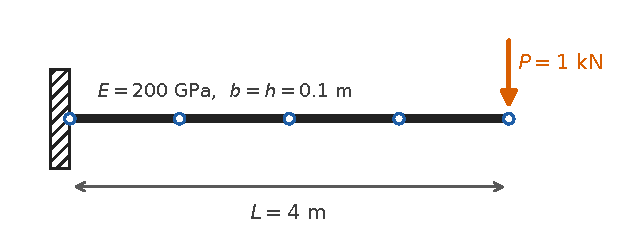
\includegraphics[width=0.85\linewidth]{../examples/voladizo_marco/fig_esquema.pdf}
\caption{Voladizo empotrado en $x = 0$ con carga puntual $P$ en el extremo libre. Los círculos marcan los cinco nodos del modelo.}
\label{fig:voladizo_marco:esquema}
\end{figure}

La viga de \hyperref[fig:voladizo_marco:esquema]{figura~\ref*{fig:voladizo_marco:esquema}} tiene longitud $L = 4$ m, está empotrada en $x = 0$ y libre en $x = L$. La sección es cuadrada, $b = h = 0.1$ m, con área $A = 0.01$ m\ensuremath{^{2}} y momento de inercia $I = bh^3/12 = 8.\overline{3}\times10^{-6}$ m⁴. El material es acero, $E = 200$ GPa. En el extremo libre actúa una carga $P = 1$ kN hacia abajo, es decir, en $-y$. Todas las magnitudes se dan en unidades SI coherentes: m, N y Pa.

\section{Solución analítica}

Con $+y$ hacia arriba y giro antihorario positivo, la teoría de Euler-Bernoulli da la deformada y el giro

\[
u_y(x) = -\frac{P\,x^2\,(3L - x)}{6EI}, \qquad
\theta(x) = \frac{du_y}{dx} = -\frac{P\,x\,(2L - x)}{2EI},
\]

de modo que en el extremo libre la flecha es $\delta = PL^3/(3EI)$ y el giro $\theta_L = -PL^2/(2EI)$, negativo porque la sección gira en sentido horario.

Las fuerzas internas se obtienen cortando la viga en $x$ y aislando el tramo derecho. En la convención de viga del programa, la cara izquierda de ese tramo (normal saliente $-x$) lleva $V$ positivo hacia $+y$ y $M$ positivo en sentido horario. El equilibrio vertical del tramo da $V - P = 0$, y el de momentos respecto al corte da $M = -P(L - x)$:

\[
N(x) = 0, \qquad V(x) = +P, \qquad M(x) = -P\,(L - x).
\]

El cortante es positivo porque tiende a girar el diferencial en sentido horario. El flector es negativo en toda la viga, lo que indica tracción en la fibra superior, como corresponde a un voladizo cargado hacia abajo. El empotramiento reacciona con $R_y = +P$ hacia arriba y con un momento $M_z = +PL$ antihorario.

\section{Modelo en Solidum}

El modelo completo es el archivo \texttt{examples/\allowbreak{}voladizo\_\allowbreak{}marco/\allowbreak{}modelo.\allowbreak{}yaml}:

\begin{lstlisting}[language=yaml]
# SOLIDUM FEM — Manual de ejemplos, ejemplo 1
# Voladizo con carga puntual en el extremo libre (marco 2D, Euler-Bernoulli)
# Unidades: m, N, Pa
#
# L = 4 m, sección cuadrada 0.1 m × 0.1 m, acero E = 200 GPa, P = 1 kN hacia abajo.
# Cuatro elementos de 1 m: con carga sólo en los nodos, la interpolación
# hermítica cúbica es la solución exacta de la ecuación de la viga, así que
# los valores nodales deben coincidir con la solución analítica a precisión
# de máquina.

nodes:
  - {id: 1, coords: [0.0, 0.0]}
  - {id: 2, coords: [1.0, 0.0]}
  - {id: 3, coords: [2.0, 0.0]}
  - {id: 4, coords: [3.0, 0.0]}
  - {id: 5, coords: [4.0, 0.0]}

materials:
  - {id: 1, type: Elastic1D, E: 200.0e9}

# A = b·h, I = b·h³/12 (m², m⁴)
elements:
  - {id: 1, type: Frame2DEuler, material: 1, nodes: [1, 2],
     A: 0.01, I: 8.333333333333e-6}
  - {id: 2, type: Frame2DEuler, material: 1, nodes: [2, 3],
     A: 0.01, I: 8.333333333333e-6}
  - {id: 3, type: Frame2DEuler, material: 1, nodes: [3, 4],
     A: 0.01, I: 8.333333333333e-6}
  - {id: 4, type: Frame2DEuler, material: 1, nodes: [4, 5],
     A: 0.01, I: 8.333333333333e-6}

# Empotramiento: desplazamientos y giro impedidos en x = 0
boundary_conditions_by_node:
  - {node_id: 1, ux: 0.0, uy: 0.0, rz: 0.0}

# P = 1 kN hacia abajo (−y) en el extremo libre
point_loads_by_node:
  - {node_id: 5, uy: -1000.0}

solver:
  type: LinearSolver

\end{lstlisting}

Los puntos que conviene notar:

\begin{itemize}
  \item \textbf{Nodos y grados de libertad.} Cada nodo de un elemento \href{https://github.com/jretamav/solidum-fem/blob/main/docs/specs/Frame2DEuler.md}{Frame2DEuler} tiene tres grados de libertad: \texttt{ux}, \texttt{uy} y \texttt{rz}. Los declara el elemento; el YAML sólo da coordenadas.
  \item \textbf{Material.} \texttt{Elastic1D} sólo necesita $E$. El área y la inercia son propiedades de la sección y van en cada elemento.
  \item \textbf{Empotramiento.} Fijar \texttt{ux}, \texttt{uy} y \texttt{rz} del nodo 1 impide los dos desplazamientos y el giro.
  \item \textbf{Carga.} \texttt{uy: -1000.0} en el nodo 5 es una fuerza de 1 kN en $-y$. Las cargas nodales se dan en ejes globales.
  \item \textbf{Solver.} \texttt{LinearSolver} resuelve $\mathbf K\,\mathbf u = \mathbf F$ una sola vez. Antes de factorizar comprueba que el modelo no sea un mecanismo, y después verifica el equilibrio de la solución.
\end{itemize}

El script \texttt{run.py} resuelve este YAML con el mismo proceso que \texttt{solidum.run\_yaml}, pero conserva el dominio para poder indexar el vector de desplazamientos por nodo (\texttt{node.dofs[\textquotedbl{}uy\textquotedbl{}]}). Las reacciones y las fuerzas internas vienen en el resultado: \texttt{res.\allowbreak{}reactions\_\allowbreak{}by\_\allowbreak{}node[1]} es un diccionario \texttt{\{\textquotedbl{}ux\textquotedbl{}: \ldots{}, \textquotedbl{}uy\textquotedbl{}: \ldots{}, \textquotedbl{}rz\textquotedbl{}: \ldots{}\}} y \texttt{res.\allowbreak{}element\_\allowbreak{}forces[e].\allowbreak{}components[\textquotedbl{}M\textquotedbl{}]} contiene el flector en los dos extremos del elemento \texttt{e}, en sus ejes locales.

\section{Resultados}

\begin{table}[h]
\centering
\caption{Voladizo de Euler-Bernoulli: Solidum frente a la solución analítica.}
\begin{tabularx}{\textwidth}{YYY}
\hline
\textbf{Magnitud} & \textbf{Solidum} & \textbf{Analítica} \\
\hline
Flecha en el extremo $\delta$ [mm] & 12.800000 & 12.800000 \\
Giro en el extremo $\theta_L$ [rad] & $-4.800000\times 10^{-3}$ & $-4.800000\times 10^{-3}$ \\
Reacción $R_y$ [N] & 1000.000000 & 1000.000000 \\
Momento de reacción $M_z$ [N\ensuremath{\cdot}m] & 4000.000000 & $PL = 4000$ \\
Flector en el empotramiento $M(0)$ [N\ensuremath{\cdot}m] & $-4000.000000$ & $-PL = -4000$ \\
Cortante $V$ [N] & 1000.000000 & 1000.000000 \\
\hline
\end{tabularx}
\end{table}
La mayor discrepancia relativa entre todas las magnitudes comparadas, incluidos los desplazamientos de los cinco nodos y las fuerzas internas en los dos extremos de cada elemento, es menor que $10^{-13}$: el redondeo de la aritmética de doble precisión.

\begin{figure}[H]
\centering
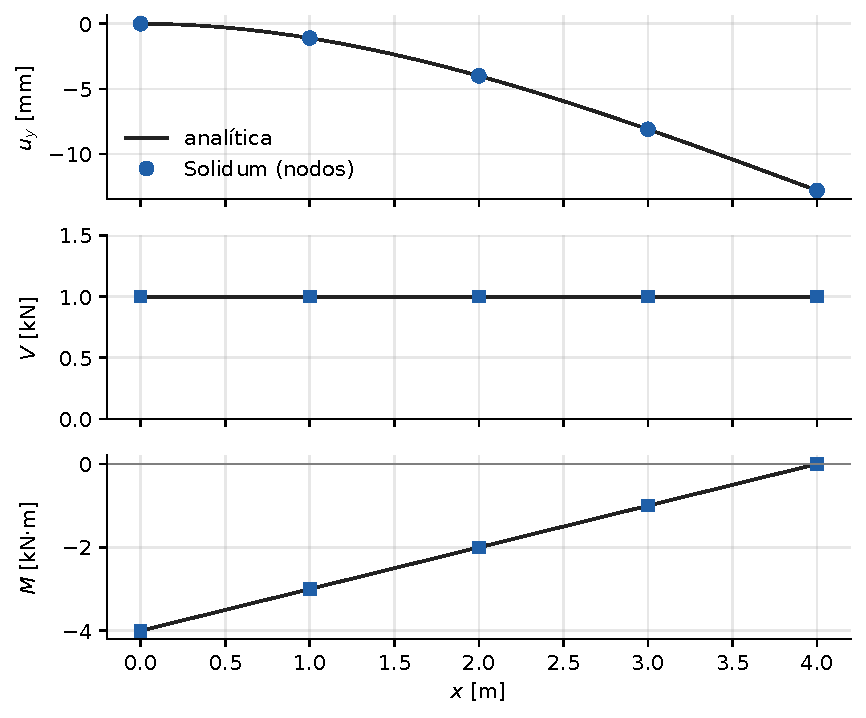
\includegraphics[width=0.8\linewidth]{../examples/voladizo_marco/fig_diagramas.pdf}
\caption{Deformada, cortante y flector del voladizo. Línea: solución analítica. Marcadores: Solidum, en los nodos (deformada) y en los dos extremos de cada elemento (fuerzas internas).}
\label{fig:voladizo_marco:diagramas}
\end{figure}

La \hyperref[fig:voladizo_marco:diagramas]{figura~\ref*{fig:voladizo_marco:diagramas}} muestra que la coincidencia no se limita al extremo. El resultado exacto tiene una explicación precisa: sin carga entre nodos, la ecuación de la viga $EI\,u_y'''' = 0$ tiene por solución un polinomio cúbico en cada tramo, y las funciones de forma hermíticas del elemento son justamente cúbicas. El método de elementos finitos reproduce entonces la solución exacta en los nodos, con cualquier número de elementos; los cuatro de este modelo sólo sirven para dibujar la deformada. Con una carga distribuida la solución exacta pasa a ser de cuarto grado y deja de estar contenida en el espacio de interpolación: los valores nodales siguen siendo exactos en el caso de la viga, pero la deformada entre nodos ya no.

Los signos de la tabla confirman la convención: el cortante sale positivo, el flector negativo (tracción arriba) y la reacción de momento positiva (antihoraria).

\section{Deformación por cortante: Timoshenko frente a Euler-Bernoulli}

La teoría de Euler-Bernoulli supone que las secciones planas permanecen perpendiculares al eje deformado y desprecia la deformación por cortante. La de Timoshenko la incluye, y la flecha en el extremo del voladizo gana un término:

\[
\delta_T = \frac{PL^3}{3EI} + \frac{PL}{\kappa G A}, \qquad
\frac{\delta_T}{\delta_{EB}} = 1 + \frac{3EI}{\kappa G A L^2},
\]

donde $\kappa A$ es el área efectiva de cortante (parámetro \texttt{As} del elemento). Para una sección rectangular, con $I/A = h^2/12$, $G = E/[2(1+\nu)]$ y $\kappa = 5/6$, el cociente depende sólo de la esbeltez:

\[
\frac{\delta_T}{\delta_{EB}} = 1 + \frac{1+\nu}{2\kappa}\left(\frac{h}{L}\right)^2
= 1 + 0.78\left(\frac{h}{L}\right)^2 \quad (\nu = 0.3).
\]

El script repite el voladizo con una sección de $0.1\times0.2$ m y esbelteces $L/h$ de 1 a 1000, cada vez con \textbf{un solo elemento} \href{https://github.com/jretamav/solidum-fem/blob/main/docs/specs/Frame2DTimoshenko.md}{Frame2DTimoshenko} y un solo Frame2DEuler. Este ejemplo usa el API de Python en vez del YAML: el modelo se construye nodo a nodo.

\begin{lstlisting}[language=Python]
def _flecha_punta(cls, L_h: float) -> float:
    """Flecha en la punta de un voladizo de un solo elemento, sección b × h = 0.1 × 0.2 m."""
    h = 0.2
    b = 0.1
    Lb = L_h * h
    A = b * h
    Ib = b * h**3 / 12.0
    domain = Domain()
    mat = Elastic1D(E=E)
    n1 = domain.add_node(1, [0.0, 0.0])
    n2 = domain.add_node(2, [Lb, 0.0])
    if cls is Frame2DTimoshenko:
        el = Frame2DTimoshenko(1, [n1, n2], mat, A=A, I=Ib, As=KAPPA * A, nu=NU)
    else:
        el = Frame2DEuler(1, [n1, n2], mat, A=A, I=Ib)
    domain.add_element(el)
    for d in ("ux", "uy", "rz"):
        n1.fix_dof(d, 0.0)
    domain.generate_equation_numbers()
    F = np.zeros(domain.total_dofs)
    F[n2.dofs["uy"]] = -P
    U = LinearSolver(Assembler(domain)).solve(F)
    return -U[n2.dofs["uy"]]

\end{lstlisting}

\begin{figure}[H]
\centering
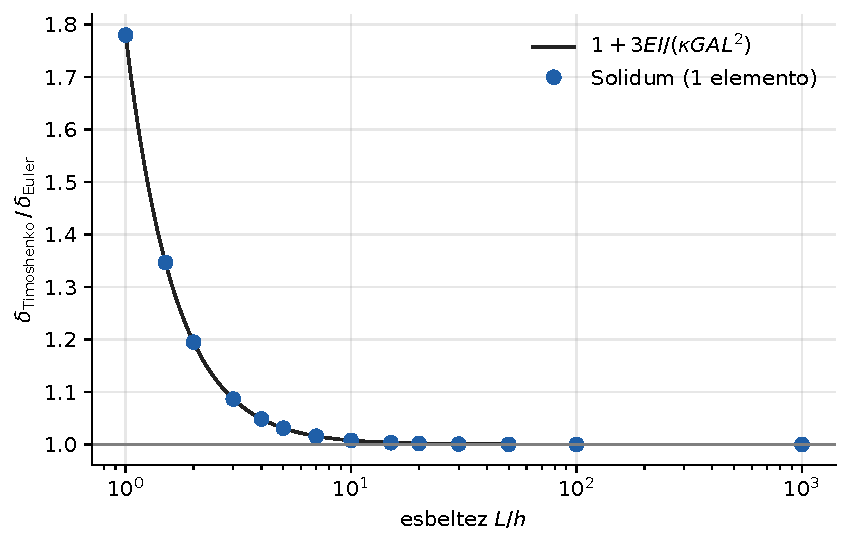
\includegraphics[width=0.9\linewidth]{../examples/voladizo_marco/fig_timoshenko.pdf}
\caption{Cociente de flechas Timoshenko / Euler-Bernoulli en función de la esbeltez. Cada punto de Solidum es un modelo de un solo elemento.}
\label{fig:voladizo_marco:timoshenko}
\end{figure}

La \hyperref[fig:voladizo_marco:timoshenko]{figura~\ref*{fig:voladizo_marco:timoshenko}} compara el cociente calculado con la expresión analítica. La discrepancia máxima es menor que $10^{-14}$. Dos lecturas prácticas:

\begin{itemize}
  \item \textbf{Cuándo importa el cortante.} En $L/h = 10$ el cortante añade un 0.78 \% a la flecha; en $L/h = 5$, un 3.12 \%; en una viga tan corta como peraltada, $L/h = 1$, la flecha es 1.78 veces la de Euler-Bernoulli. La regla habitual de usar Timoshenko por debajo de $L/h \approx 10$ sale directamente de esta curva.
  \item \textbf{Sin bloqueo por cortante.} En $L/h = 1000$ el cociente excede la unidad en $7.8\times 10^{-7}$, como predice la teoría. Un elemento de Timoshenko con interpolación lineal independiente de flecha y giro, integrado de forma completa, se bloquea en ese límite: su rigidez a cortante domina y la flecha tiende a cero en vez de tender a la de Euler-Bernoulli. Frame2DTimoshenko usa la rigidez exacta de la viga de Timoshenko, escrita con el factor $\Phi = 12EI/(\kappa G A L^2)$; equivale a funciones de forma que dependen de $\Phi$ y se reducen a las hermíticas cuando $\Phi \to 0$. Por eso un elemento basta a cualquier esbeltez.
\end{itemize}

\section{Para seguir}

\begin{itemize}
  \item Cambiar un elemento del YAML por \texttt{Frame2DTimoshenko}, con \texttt{As: 0.00833333} y \texttt{nu: 0.3}. Como el cortante es constante, la flecha en el extremo debe crecer en $P\ell/(\kappa G A)$, con $\ell = 1$ m la longitud del tramo cambiado.
  \item Añadir peso propio con el bloque \texttt{gravity} y la \texttt{density} del material. La carga distribuida hace que el flector entre nodos sea parabólico; los valores de extremo de \texttt{element\_forces} descuentan la carga nodal equivalente y siguen siendo exactos.
  \item El mismo voladizo modelado con sólidos 2D de cuatro nodos muestra el bloqueo por cortante que aquí no aparece. Lo documenta el benchmark de MacNeal-Harder en \texttt{tests/\allowbreak{}validation/\allowbreak{}test\_\allowbreak{}slender\_\allowbreak{}cantilever.\allowbreak{}py}.
\end{itemize}

\textbf{Archivos del ejemplo.} La carpeta \texttt{examples/\allowbreak{}voladizo\_\allowbreak{}marco/\allowbreak{}} contiene el modelo \texttt{modelo.yaml}, el script \texttt{run.py}, los resultados en \texttt{resultados.json} y las figuras. Para regenerar resultados y figuras basta con ejecutar el script.


\newpage

\chapter{Placa con agujero a tracción: concentración de esfuerzos de Kirsch}
\chaptermark{Placa con agujero a tracción}
\label{cap:placa_agujero_kirsch}





Un agujero circular en una placa traccionada multiplica por tres el esfuerzo en su borde. Es el caso clásico de concentración de esfuerzos, resuelto por Kirsch en 1898 para una placa infinita, y el primer problema bidimensional de este manual. A diferencia del voladizo, aquí la solución de elementos finitos ya no es exacta: el ejemplo enseña a medir cuánto se aparta de la analítica, dónde y por qué.

\textbf{Qué se aprende}

\begin{itemize}
  \item Resolver una malla de Gmsh desde el YAML y aplicar condiciones de contorno por grupo físico.
  \item Aprovechar la doble simetría para modelar sólo un cuarto de la placa.
  \item Cargar con desplazamiento impuesto y obtener el esfuerzo nominal a partir de la reacción.
  \item Leer esfuerzos en los puntos de Gauss y recuperarlos en los nodos.
  \item Graduar la malla hacia el concentrador de esfuerzos.
  \item Distinguir el error de discretización, que baja al refinar, del error de modelo, que no.
\end{itemize}

\section{Planteamiento}

Una placa de acero con un agujero de radio $a = 10$ mm se tracciona en la dirección $x$. Lejos del agujero el esfuerzo es uniaxial y uniforme, $\sigma_{xx} = \sigma_\infty$. La placa es delgada, con espesor de 10 mm, y trabaja en esfuerzo plano, con $E = 200$ GPa y $\nu = 0.3$.

El problema es simétrico respecto a los ejes $x$ e $y$, así que basta con el cuarto $x \ge 0$, $y \ge 0$. En los bordes de simetría se impone desplazamiento normal nulo: $u_x = 0$ sobre $x = 0$ y $u_y = 0$ sobre $y = 0$. El cuarto de placa mide $W = H = 20a$, lo bastante grande para que los bordes apenas perturben el campo del agujero.

\begin{figure}[H]
\centering
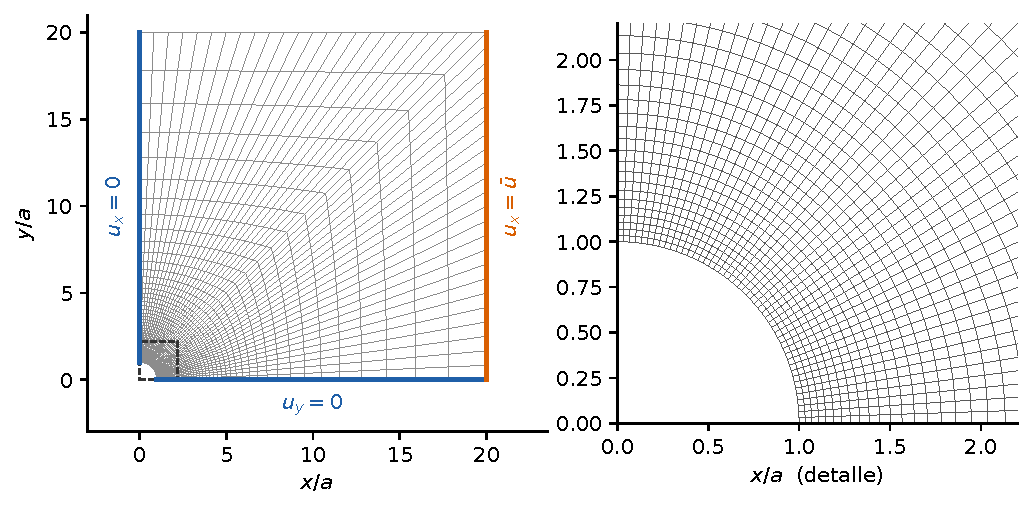
\includegraphics[width=0.9\linewidth]{../examples/placa_agujero_kirsch/fig_malla.pdf}
\caption{Cuarto de placa modelado: malla estructurada de cuadriláteros, condiciones de simetría (azul) y desplazamiento impuesto (naranja). A la derecha, el detalle marcado junto al agujero.}
\label{fig:placa_agujero_kirsch:malla}
\end{figure}

\section{Solución analítica}

Para una placa infinita con un agujero libre de tracción, en coordenadas polares $(r, \theta)$ con $\theta$ medido desde el eje $x$, Kirsch obtuvo

\[
\begin{aligned}
\sigma_{rr} &= \frac{\sigma_\infty}{2}\left(1 - \frac{a^2}{r^2}\right)
 + \frac{\sigma_\infty}{2}\left(1 - \frac{4a^2}{r^2} + \frac{3a^4}{r^4}\right)\cos 2\theta,\\
\sigma_{\theta\theta} &= \frac{\sigma_\infty}{2}\left(1 + \frac{a^2}{r^2}\right)
 - \frac{\sigma_\infty}{2}\left(1 + \frac{3a^4}{r^4}\right)\cos 2\theta,\\
\sigma_{r\theta} &= -\frac{\sigma_\infty}{2}\left(1 + \frac{2a^2}{r^2} - \frac{3a^4}{r^4}\right)\sin 2\theta .
\end{aligned}
\]

En el borde del agujero sólo queda el esfuerzo circunferencial, $\sigma_{\theta\theta}(a, \theta) = \sigma_\infty\,(1 - 2\cos 2\theta)$. Vale $3\sigma_\infty$ en $\theta = 90°$, el punto $(0, a)$, y $-\sigma_\infty$ en $\theta = 0$: el borde del agujero se comprime en la dirección transversal a la carga. Sobre el eje $x = 0$,

\[
\sigma_{xx}(0, y) = \sigma_\infty\left(1 + \frac{a^2}{2y^2} + \frac{3a^4}{2y^4}\right),
\]

que decae de $3\sigma_\infty$ a $\sigma_\infty$ en pocos radios. El factor de concentración de esfuerzos es $K_t = \sigma_{xx}(0, a)/\sigma_\infty = 3$, independiente del tamaño del agujero y del material.

\section{Modelo en Solidum}

\textbf{La malla.} El script \texttt{malla.py} genera la malla con el API de Python de Gmsh y la guarda en \texttt{placa\_\allowbreak{}agujero.\allowbreak{}msh}, que se versiona junto al ejemplo; resolverlo no requiere Gmsh. La malla es estructurada y tiene dos zonas. Hasta $r = 5a$ es un anillo polar: líneas radiales rectas y circunferencias concéntricas, con elementos que crecen en progresión geométrica desde el agujero, donde el gradiente de esfuerzos es fuerte. De ahí al contorno, dos parches de transición. Todos los elementos son cuadriláteros \href{https://github.com/jretamav/solidum-fem/blob/main/docs/specs/Quad4.md}{Quad4}. La malla define grupos físicos con nombre (\texttt{Simetria\_X}, \texttt{Simetria\_Y}, \texttt{Borde\_Carga}, \texttt{Agujero}), y el YAML los usa para aplicar las condiciones de contorno.

\textbf{La carga.} El YAML de Solidum todavía no admite tracciones distribuidas sobre un borde; el API de Python sí, con el método \texttt{compute\_\allowbreak{}edge\_\allowbreak{}traction} de los elementos sólidos. Aquí la carga es un desplazamiento impuesto $\bar u = 0.1$ mm en todo el borde $x = W$, como el que aplican las mordazas de una máquina de ensayo. El esfuerzo nominal lejano se obtiene después: $\sigma_\infty = R_x/(H\,t)$, con $R_x$ la reacción total en ese borde.

\begin{lstlisting}[language=yaml]
# SOLIDUM FEM — Manual de ejemplos, ejemplo 2
# Placa con agujero circular a tracción: concentración de esfuerzos (Kirsch)
# Unidades: m, N, Pa
#
# Cuarto de placa por doble simetría: agujero de radio a = 10 mm, placa de
# 200 mm × 200 mm (20a × 20a), espesor 10 mm, acero en esfuerzo plano.
# La carga se aplica como desplazamiento impuesto en x = W; el esfuerzo
# nominal σ∞ se obtiene después de la reacción total en ese borde.

mesh: placa_agujero.msh      # generada por malla.py (Gmsh), Quad4
mesh_material: 1
mesh_thickness: 0.01

materials:
  - {id: 1, type: Elastic2D, E: 200.0e9, nu: 0.3, hypothesis: plane_stress}

boundary_conditions_by_group:
  - {group_name: "Simetria_X", ux: 0.0}      # x = 0: simetría respecto al eje y
  - {group_name: "Simetria_Y", uy: 0.0}      # y = 0: simetría respecto al eje x
  - {group_name: "Borde_Carga", ux: 1.0e-4}  # x = W: alargamiento impuesto de 0.1 mm

solver:
  type: LinearSolver

\end{lstlisting}

\textbf{Los esfuerzos.} El método de desplazamientos da los esfuerzos con más precisión en los puntos de Gauss que en los nodos. El script los evalúa en los cuatro puntos de Gauss de cada elemento con \texttt{gauss\_states} y compara cada uno con el campo de Kirsch en ese mismo punto. Para los valores en la frontera, como $K_t$ o el esfuerzo en el borde del agujero, los extrapola a los nodos con el campo bilineal que pasa por los cuatro valores de Gauss y promedia entre los elementos que comparten el nodo. Es la recuperación nodal habitual de los programas comerciales. La función \texttt{calcular} de \texttt{run.py} hace todo el recorrido:

\begin{lstlisting}[language=Python]
def calcular() -> dict:
    domain, _, res = resolver_yaml_estatico(AQUI / "modelo.yaml")

    # Esfuerzo nominal lejano: reacción total en el borde cargado / área.
    grupo = domain.physical_groups
    rx = sum(res.reactions_by_node[n]["ux"] for n in grupo["Borde_Carga"])
    s_inf = rx / (H * ESPESOR)

    # Puntos de Gauss: Solidum frente a Kirsch en el mismo punto.
    estados = gauss_states(domain, res.U)
    pts = np.vstack([gs["points_global"] for gs in estados.values()])
    sig = np.vstack([gs["stress"] for gs in estados.values()])
    sk = np.column_stack(kirsch(pts[:, 0], pts[:, 1], s_inf))
    err_pg = np.abs(sig - sk).max(axis=1) / s_inf
    r_pg = np.hypot(pts[:, 0], pts[:, 1])
    cercano = r_pg <= R_CERCANO
    lejano = r_pg > R_LEJANO

    # Esfuerzos nodales recuperados: línea x = 0 y borde del agujero.
    nodal = esfuerzos_nodales(domain, estados)
    coords = {nid: np.asarray(domain.nodes[nid].coordinates) for nid in nodal}

    eje = sorted(grupo["Simetria_X"], key=lambda n: coords[n][1])
    y_eje = np.array([coords[n][1] for n in eje])
    sxx_eje = np.array([nodal[n][0] for n in eje])

    borde = sorted(grupo["Agujero"], key=lambda n: np.arctan2(coords[n][1], coords[n][0]))
    th = np.array([np.arctan2(coords[n][1], coords[n][0]) for n in borde])
    s_b = np.array([nodal[n] for n in borde])
    c, s = np.cos(th), np.sin(th)
    stt_b = s_b[:, 0] * s**2 + s_b[:, 1] * c**2 - 2 * s_b[:, 2] * s * c
    stt_k = s_inf * (1 - 2 * np.cos(2 * th))

    kt = sxx_eje[0] / s_inf        # nodo (0, a): primero de la línea x = 0
    return {
        "a": A, "W": W, "H": H, "espesor": ESPESOR,
        "n_elementos": len(domain.elements), "n_nodos": len(domain.nodes),
        "n_puntos_gauss": int(len(pts)), "n_puntos_cercanos": int(cercano.sum()),
        "reaccion_total": rx, "sigma_inf": s_inf, "sigma_inf_MPa": s_inf / 1e6,
        "Kt": kt, "error_Kt": error_relativo(kt, 3.0),
        "error_Kt_pct": 100 * (kt - 3.0) / 3.0,
        "sigma_min_borde": float(stt_b.min() / s_inf),
        "error_borde_max": float(np.abs(stt_b - stt_k).max() / s_inf),
        "error_borde_max_pct": float(100 * np.abs(stt_b - stt_k).max() / s_inf),
        "error_gauss_cercano": float(err_pg[cercano].max()),
        "error_gauss_cercano_pct": float(100 * err_pg[cercano].max()),
        "rms_gauss_cercano": float(np.sqrt(np.mean(err_pg[cercano] ** 2))),
        "rms_gauss_cercano_pct": float(100 * np.sqrt(np.mean(err_pg[cercano] ** 2))),
        "error_gauss_lejano": float(err_pg[lejano].max()),
        "error_gauss_lejano_pct": float(100 * err_pg[lejano].max()),
        "primer_elemento_radial_sobre_a": float(
            (np.sort(np.hypot(*np.array([domain.nodes[n].coordinates
                                         for n in grupo["Simetria_Y"]]).T))[1] - A) / A),
        "eje_y": y_eje, "eje_sxx": sxx_eje,
        "borde_theta": th, "borde_stt": stt_b,
    }

\end{lstlisting}

\section{Resultados}

La reacción da $\sigma_\infty =$ 99.41 MPa, algo menos que los 100 MPa de $E\,\bar u/W$, porque el agujero hace a la placa ligeramente más flexible.

\begin{table}[h]
\centering
\caption{Placa con agujero: Solidum frente a Kirsch. Errores relativos a $\sigma_\infty$.}
\begin{tabularx}{\textwidth}{YYY}
\hline
\textbf{Magnitud} & \textbf{Solidum} & \textbf{Kirsch} \\
\hline
Factor de concentración $K_t$ & 3.026 & 3 \\
Mínimo de $\sigma_{\theta\theta}/\sigma_\infty$ en el borde & $-1.011$ & $-1$ \\
Error máximo de $\sigma_{\theta\theta}$ en el borde & 2.6 \% & --- \\
Error máximo en puntos de Gauss con $r \le 2a$ & 7.5 \% & --- \\
Error medio cuadrático en puntos de Gauss con $r \le 2a$ & 2.2 \% & --- \\
Error máximo en puntos de Gauss con $r > 5a$ & 1.0 \% & --- \\
\hline
\end{tabularx}
\end{table}
\begin{figure}[H]
\centering
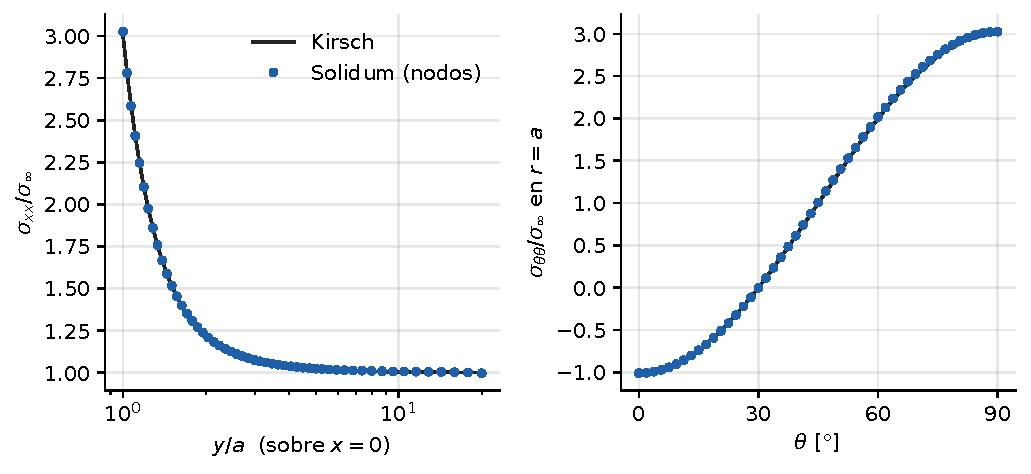
\includegraphics[width=0.9\linewidth]{../examples/placa_agujero_kirsch/fig_kirsch.pdf}
\caption{Izquierda: $\sigma_{xx}$ sobre el eje $x = 0$. Derecha: esfuerzo circunferencial en el borde del agujero. Marcadores: valores nodales recuperados de Solidum.}
\label{fig:placa_agujero_kirsch:kirsch}
\end{figure}

La \hyperref[fig:placa_agujero_kirsch:kirsch]{figura~\ref*{fig:placa_agujero_kirsch:kirsch}} muestra las dos distribuciones que interesan en diseño. El esfuerzo sobre el eje de simetría decae de tres veces el nominal a prácticamente el nominal en unos cuatro radios, y la concentración es local. En el borde, el esfuerzo circunferencial recorre la curva $1 - 2\cos 2\theta$ entre la compresión en $\theta = 0$ y el máximo en $\theta = 90°$. El factor de concentración calculado, 3.026, está un 0.9 \% por encima de 3.

\begin{figure}[H]
\centering
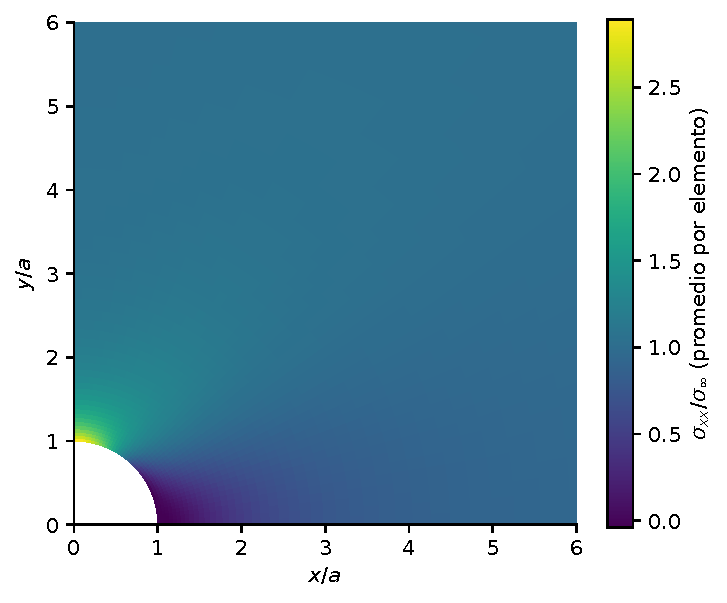
\includegraphics[width=0.58\linewidth]{../examples/placa_agujero_kirsch/fig_campo.pdf}
\caption{Campo de $\sigma_{xx}/\sigma_\infty$ cerca del agujero, promedio por elemento.}
\label{fig:placa_agujero_kirsch:campo}
\end{figure}

\section{Dos fuentes de error}

Los errores de la tabla no tienen un solo origen, y separarlos es lo que este ejemplo enseña.

\begin{itemize}
  \item \textbf{Error de discretización.} Es el mayor, y se concentra junto al agujero, donde el esfuerzo varía más rápido. Un Quad4 representa los esfuerzos sólo de forma aproximadamente lineal dentro de cada elemento, y junto al agujero $\sigma_{xx}$ cae a la mitad en medio radio. Por eso el primer anillo de elementos tiene un espesor radial de sólo 0.034$\,a$. Este error baja al refinar: al duplicar la densidad de la malla, el error en los puntos de Gauss cercanos se reduce a la mitad y $K_t$ se acerca a 3. El ejemplo 3 estudia esa convergencia en detalle.
  \item \textbf{Error de modelo.} Lejos del agujero el error se estanca en torno al 1 \%, y refinar no lo reduce. Kirsch supone una placa infinita traccionada por un esfuerzo uniforme; el modelo es una placa finita de $20a \times 20a$ cuyo borde se desplaza uniformemente. Un desplazamiento uniforme no produce una tracción uniforme cuando el agujero perturba el campo. Las dos soluciones responden a problemas distintos, y la diferencia no es un error del programa.
\end{itemize}

La calidad de la malla también cuenta. Una primera versión de este ejemplo usaba dos parches transfinitos desde el agujero hasta el contorno, sin anillo polar. Sus líneas circunferenciales quedaban quebradas sobre la diagonal y los errores junto a ella eran bastante mayores. El anillo polar mantiene los elementos casi rectangulares donde más importa.

\section{Para seguir}

\begin{itemize}
  \item Refinar la malla cambiando \texttt{N\_ARCO}, \texttt{N\_ANILLO} y \texttt{N\_EXT} en \texttt{malla.py}, regenerarla y volver a resolver: $K_t$ debe acercarse a 3 y el error junto al agujero debe bajar a la mitad con cada duplicación.
  \item Agrandar la placa, con \texttt{W} y \texttt{H}, para ver cómo baja el error lejano.
  \item Cambiar el agujero por una elipse de semiejes $b$ en $x$ y $c$ en $y$, y comparar con la solución de Inglis, $K_t = 1 + 2c/b$.
\end{itemize}

\textbf{Archivos del ejemplo.} La carpeta \texttt{examples/\allowbreak{}placa\_\allowbreak{}agujero\_\allowbreak{}kirsch/\allowbreak{}} contiene el generador de malla \texttt{malla.py}, la malla \texttt{placa\_\allowbreak{}agujero.\allowbreak{}msh}, el modelo \texttt{modelo.yaml}, el script \texttt{run.py}, los resultados en \texttt{resultados.json} y las figuras.


\newpage

\chapter{Cilindro de pared gruesa: estudio de convergencia con el API de Python}
\chaptermark{Cilindro de pared gruesa}
\label{cap:cilindro_lame}





Un modelo de elementos finitos converge a la solución exacta cuando la malla se refina, y lo hace con una rapidez que la teoría predice para cada elemento. Este ejemplo lo comprueba en el cilindro de pared gruesa bajo presión interna, cuya solución cerrada se debe a Lamé. El modelo se construye con el API de Python, sin YAML, lo que permite generar las mallas y repetir el cálculo en un bucle.

\textbf{Qué se aprende}

\begin{itemize}
  \item Construir un modelo sólido 2D con el API: nodos, elementos, material y apoyos.
  \item Aplicar una presión sobre un contorno curvo con su vector de cargas consistente.
  \item Medir errores contra una solución analítica y estimar el orden de convergencia.
  \item Por qué el esfuerzo converge un orden más despacio que el desplazamiento.
  \item Cuánto más rinden los elementos cuadráticos que los lineales por grado de libertad.
\end{itemize}

\section{Planteamiento}

Un tubo largo de acero, con radio interior $R_i = 100$ mm y exterior $R_e = 200$ mm, soporta una presión interna $p = 10$ MPa. Por ser largo y estar impedido axialmente, trabaja en deformación plana. El material tiene $E = 200$ GPa y $\nu = 0.3$. Por simetría se modela un cuarto de la sección, con $u_y = 0$ sobre el eje $x$ y $u_x = 0$ sobre el eje $y$.

\begin{figure}[H]
\centering
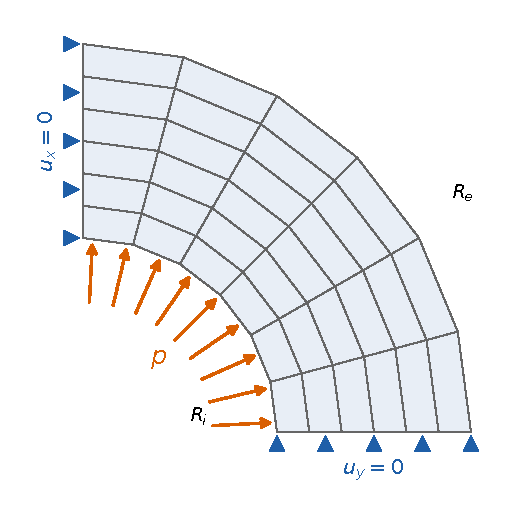
\includegraphics[width=0.55\linewidth]{../examples/cilindro_lame/fig_esquema.pdf}
\caption{Cuarto de sección modelado, con una malla de $6 \times 6$ cuadriláteros. La presión actúa sobre el contorno interior.}
\label{fig:cilindro_lame:esquema}
\end{figure}

\section{Solución analítica}

La solución de Lamé en coordenadas polares es

\[
\sigma_{rr} = A - \frac{B}{r^2}, \qquad
\sigma_{\theta\theta} = A + \frac{B}{r^2}, \qquad
A = \frac{p R_i^2}{R_e^2 - R_i^2}, \quad B = \frac{p R_i^2 R_e^2}{R_e^2 - R_i^2},
\]

y, en deformación plana,

\[
u_r = \frac{1+\nu}{E}\left[(1 - 2\nu)\,A\,r + \frac{B}{r}\right], \qquad
\sigma_{zz} = \nu\,(\sigma_{rr} + \sigma_{\theta\theta}) = 2\nu A .
\]

El esfuerzo circunferencial es máximo en la cara interior, $\sigma_{\theta\theta}(R_i) =$ 16.67 MPa, y el desplazamiento radial allí vale 9.533 \ensuremath{\mu}m. El esfuerzo axial $\sigma_{zz}$ es constante: Solidum lo calcula en el material, aunque el modelo 2D no lo muestra entre sus tres componentes.

\section{Modelo con el API de Python}

La función \texttt{modelo} construye el cuarto de corona con $n \times n$ celdas en $(r, \theta)$ y cualquiera de los cuatro elementos del estudio: \href{https://github.com/jretamav/solidum-fem/blob/main/docs/specs/Tri3.md}{Tri3} y Quad4, lineales, y Tri6 y \href{https://github.com/jretamav/solidum-fem/blob/main/docs/specs/Quad8.md}{Quad8}, cuadráticos. Los nodos intermedios de los elementos cuadráticos quedan sobre las circunferencias, así que su contorno interior es curvo; el de los lineales es un polígono inscrito.

\begin{lstlisting}[language=Python]
def modelo(nombre: str, n: int, material=None, cuadratura: str | None = None):
    """Cuarto de corona con n × n celdas de ``nombre``. Devuelve el dominio,
    las aristas cargadas ``[(elemento, arista)]`` y los nodos. Por omisión,
    acero elástico en deformación plana y la cuadratura propia de cada
    elemento (el ejemplo 4 pasa un material plástico y, para el Quad8,
    integración reducida ``"2x2"``)."""
    cls = CLASES[nombre]
    cuadratico = nombre in ("Tri6", "Quad8")
    k = 2 if cuadratico else 1          # nodos por celda en cada dirección
    ni = nj = k * n + 1
    if material is None:
        material = Elastic2D(E=E, nu=NU, hypothesis="plane_strain")
    domain = Domain()
    nodo = {}
    for j in range(nj):
        th = 0.5 * np.pi * j / (nj - 1)
        for i in range(ni):
            if nombre == "Quad8" and i % 2 == 1 and j % 2 == 1:
                continue                    # Quad8 no tiene nodo central
            r = RI + (RE - RI) * i / (ni - 1)
            nodo[i, j] = domain.add_node(len(nodo) + 1, [r * np.cos(th), r * np.sin(th)])

    aristas = []
    for cj in range(n):
        for ci in range(n):
            i, j = k * ci, k * cj
            c1, c2, c3, c4 = nodo[i, j], nodo[i + k, j], nodo[i + k, j + k], nodo[i, j + k]
            eid = len(domain.elements) + 1
            if nombre == "Quad4":
                el = [cls(eid, [c1, c2, c3, c4], material, thickness=1.0,
                          quadrature=cuadratura)]
                cara = (el[0], 3)                          # arista c4 → c1, en r = RI
            elif nombre == "Quad8":
                m = [nodo[i + 1, j], nodo[i + 2, j + 1], nodo[i + 1, j + 2], nodo[i, j + 1]]
                el = [cls(eid, [c1, c2, c3, c4] + m, material, thickness=1.0,
                          quadrature=cuadratura)]
                cara = (el[0], 3)
            elif nombre == "Tri3":
                el = [cls(eid, [c1, c2, c3], material, thickness=1.0),
                      cls(eid + 1, [c1, c3, c4], material, thickness=1.0)]
                cara = (el[1], 2)                          # arista c4 → c1
            else:                                          # Tri6
                cen = nodo[i + 1, j + 1]
                el = [cls(eid, [c1, c2, c3, nodo[i + 1, j], nodo[i + 2, j + 1], cen],
                          material, thickness=1.0),
                      cls(eid + 1, [c1, c3, c4, cen, nodo[i + 1, j + 2], nodo[i, j + 1]],
                          material, thickness=1.0)]
                cara = (el[1], 2)
            for e in el:
                domain.add_element(e)
            if ci == 0:
                aristas.append(cara)

    for i in range(ni):                    # simetría
        if (i, 0) in nodo:
            nodo[i, 0].fix_dof("uy", 0.0)
        if (i, nj - 1) in nodo:
            nodo[i, nj - 1].fix_dof("ux", 0.0)
    domain.generate_equation_numbers()
    return domain, aristas, nodo

\end{lstlisting}

\textbf{La presión.} El método \texttt{compute\_\allowbreak{}edge\_\allowbreak{}traction} de los elementos sólidos integra una tracción de dirección constante sobre una arista. Una presión no lo es: empuja en la dirección normal al contorno, que cambia a lo largo de una arista curva. La función \texttt{carga\_de\_presion} integra $\int_\Gamma \mathbf N^\top (-p\,\mathbf n)\,d\Gamma$ con tres puntos de Gauss sobre la geometría de cada arista, recta o parabólica:

\begin{lstlisting}[language=Python]
def carga_de_presion(domain, aristas, p: float) -> np.ndarray:
    """Vector de cargas consistente con una presión ``p`` sobre las aristas.

    La presión empuja contra la cara: t = −p n, con n la normal exterior del
    sólido. Se integra ∫ Nᵀ t dΓ sobre la geometría discretizada de cada
    arista (recta o parabólica), con tres puntos de Gauss: n varía a lo largo
    de una arista curva, así que no sirve una tracción constante.
    """
    F = np.zeros(domain.total_dofs)
    xg, wg = np.polynomial.legendre.leggauss(3)
    for el, arista in aristas:
        loc = el.EDGE_NODES[arista]
        X = np.array([el.nodes[q].coordinates[:2] for q in loc], dtype=float)
        dofs = el.get_global_dof_indices()
        for s, w in zip(xg, wg):
            if len(loc) == 2:
                N = np.array([(1 - s) / 2, (1 + s) / 2])
                dN = np.array([-0.5, 0.5])
            else:                                          # (extremo, medio, extremo)
                N = np.array([s * (s - 1) / 2, 1 - s**2, s * (s + 1) / 2])
                dN = np.array([s - 0.5, -2 * s, s + 0.5])
            dx, dy = dN @ X
            # Recorriendo la arista en el sentido del elemento (antihorario), la
            # normal exterior multiplicada por |J| es (dy, −dx).
            t = -p * np.array([dy, -dx])
            for a, q in enumerate(loc):
                for d in range(2):
                    g = dofs[2 * q + d]
                    if g >= 0:
                        F[g] += w * N[a] * t[d] * el.thickness
    return F

\end{lstlisting}

Con el dominio y la carga, resolver es una línea: \texttt{LinearSolver(Assembler(domain)).\allowbreak{}solve(F)} devuelve el vector de desplazamientos.

\section{Estudio de convergencia}

Cada elemento se resuelve en mallas de $2 \times 2$ a $64 \times 64$ celdas para los lineales, y hasta $32 \times 32$ para los cuadráticos, que llegan antes a errores muy pequeños. Se miden dos errores relativos:

\begin{itemize}
  \item en desplazamientos, la media cuadrática del error de $u_r$ en todos los nodos;
  \item en esfuerzos, la media cuadrática del error de $(\sigma_{rr}, \sigma_{\theta\theta})$ en todos los puntos de Gauss.
\end{itemize}

Si el error se comporta como $e \approx C\,h^k$, en escala logarítmica es una recta de pendiente $k$, el \textbf{orden de convergencia}. La teoría del método predice, para una interpolación de grado $p$, orden $p+1$ en desplazamientos y $p$ en esfuerzos: los esfuerzos salen de derivar los desplazamientos y pierden un orden.

\begin{figure}[H]
\centering
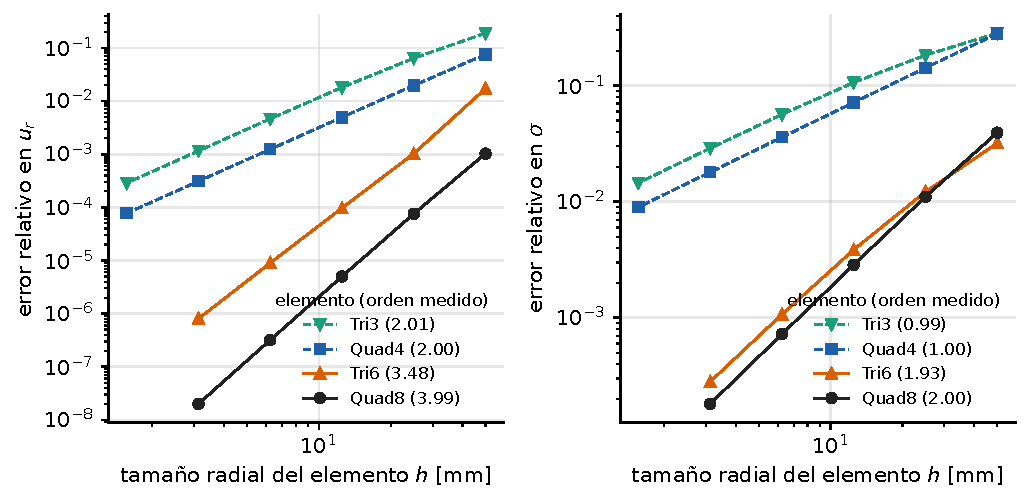
\includegraphics[width=0.9\linewidth]{../examples/cilindro_lame/fig_convergencia.pdf}
\caption{Error relativo frente al tamaño radial del elemento. Entre paréntesis, la pendiente medida entre las dos mallas más finas.}
\label{fig:cilindro_lame:convergencia}
\end{figure}

\begin{table}[h]
\centering
\caption{Órdenes de convergencia medidos entre las dos mallas más finas y órdenes teóricos.}
\begin{tabularx}{\textwidth}{YYYYYY}
\hline
\textbf{Elemento} & \textbf{$p$} & \textbf{Desplazamiento, medido} & \textbf{Desplazamiento, teórico} & \textbf{Esfuerzo, medido} & \textbf{Esfuerzo, teórico} \\
\hline
Tri3 & 1 & 2.01 & 2 & 0.99 & 1 \\
Quad4 & 1 & 2.00 & 2 & 1.00 & 1 \\
Tri6 & 2 & 3.48 & 3 & 1.93 & 2 \\
Quad8 & 2 & 3.99 & 3 & 2.00 & 2 \\
\hline
\end{tabularx}
\end{table}
Los esfuerzos convergen con el orden teórico en los cuatro elementos. Los desplazamientos lo alcanzan o lo superan. El Quad8 llega a orden 4: en mallas regulares, los valores nodales de algunos elementos convergen más rápido que el campo en su conjunto, un fenómeno conocido como \textbf{superconvergencia}. La teoría garantiza el orden $p+1$; lo que se mide por encima es un regalo de la regularidad de la malla, con el que no conviene contar en mallas arbitrarias.

\section{Lineales frente a cuadráticos}

La \hyperref[fig:cilindro_lame:convergencia]{figura~\ref*{fig:cilindro_lame:convergencia}} muestra la diferencia práctica. Con la malla de $8 \times 8$ celdas, el error en esfuerzos del Quad4 es 7.2 \% y el del Quad8 0.29 \%. Con la malla más fina, de 8450 grados de libertad, el Quad4 todavía queda en 0.90 \%, peor que el Quad8 de $8 \times 8$ con sólo 450 grados de libertad. Cuando el campo de esfuerzos es suave, los elementos cuadráticos alcanzan una precisión dada con muchos menos grados de libertad.

\begin{figure}[H]
\centering
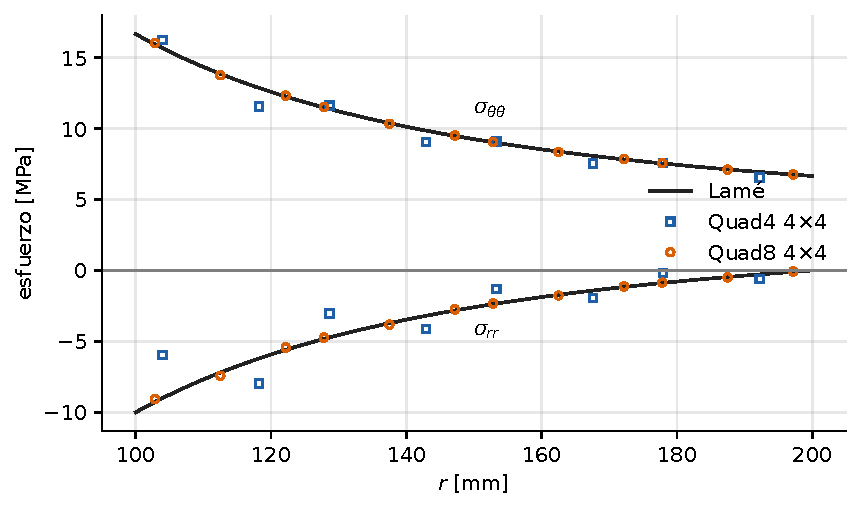
\includegraphics[width=0.9\linewidth]{../examples/cilindro_lame/fig_perfiles.pdf}
\caption{Esfuerzos en los puntos de Gauss con una malla de $4 \times 4$ celdas.}
\label{fig:cilindro_lame:perfiles}
\end{figure}

La \hyperref[fig:cilindro_lame:perfiles]{figura~\ref*{fig:cilindro_lame:perfiles}} explica el motivo. Con cuatro Quad4 en el espesor, el esfuerzo de cada elemento no puede seguir la variación $1/r^2$: sus puntos se dispersan alrededor de la curva, sobre todo en $\sigma_{rr}$ cerca de la cara interior. El Quad8, cuyo esfuerzo varía linealmente dentro del elemento, reproduce la solución con la misma malla.

\section{Para seguir}

\begin{itemize}
  \item Repetir el estudio con $\nu = 0.4999$. En deformación plana, casi incompresible, los elementos lineales con integración completa sufren \textbf{bloqueo volumétrico}: el error en desplazamientos crece mucho y la solución sale demasiado rígida.
  \item Adaptar la función \texttt{modelo} al Quad9, que añade al Quad8 el nodo central de cada celda, y comparar ambos.
  \item Distorsionar la malla desplazando al azar los nodos interiores. ¿Se mantienen los órdenes medidos? ¿Y la superconvergencia del Quad8?
\end{itemize}

\textbf{Archivos del ejemplo.} La carpeta \texttt{examples/\allowbreak{}cilindro\_\allowbreak{}lame/\allowbreak{}} contiene el script \texttt{run.py}, que genera las mallas, los resultados en \texttt{resultados.json} y las figuras.


\newpage

\chapter{Cilindro elastoplástico: primera fluencia, colapso y bloqueo volumétrico}
\chaptermark{Cilindro elastoplástico}
\label{cap:cilindro_elastoplastico}





El cilindro del ejemplo anterior, ahora de un material que fluye. Al aumentar la presión, la cara interior plastifica primero; la zona plástica avanza hacia fuera y, cuando alcanza la cara exterior, el tubo ya no admite más presión: ha llegado al colapso plástico. Las dos presiones que marcan ese recorrido tienen expresión cerrada, y el ejemplo las usa para verificar el material de von Mises, el solver de longitud de arco y el comportamiento de cinco elementos en régimen plástico.

\textbf{Qué se aprende}

\begin{itemize}
  \item Usar un material elastoplástico (\texttt{VonMises2D}) en deformación plana.
  \item Trazar una curva presión-desplazamiento con el método de longitud de arco, que puede seguir la meseta del colapso.
  \item Declarar el primer paso como fracción de la carga, sin conocer de antemano los desplazamientos.
  \item Reconocer el \textbf{bloqueo volumétrico} en plasticidad y evitarlo con la elección del elemento.
\end{itemize}

\section{Planteamiento}

La geometría, la malla y la carga son las del ejemplo 3: radio interior $a = 100$ mm, exterior $b = 200$ mm, un cuarto de sección por simetría y presión interna $p$. El acero es ahora elastoplástico perfecto, sin endurecimiento: $E = 200$ GPa, $\nu = 0.3$ y esfuerzo de fluencia $\sigma_y =$ 240 MPa, con el criterio de von Mises. El tubo trabaja en deformación plana.

\section{Soluciones analíticas}

\textbf{Primera fluencia.} Mientras el material es elástico vale la solución de Lamé. El esfuerzo equivalente de von Mises es máximo en la cara interior, donde, con $\sigma_{zz} = \nu(\sigma_{rr} + \sigma_{\theta\theta})$,

\[
\sigma_{eq}(a) = \frac{p}{b^2 - a^2}\sqrt{3\,b^4 + (1 - 2\nu)^2\,a^4},
\qquad
p_e = \sigma_y\,\frac{b^2 - a^2}{\sqrt{3\,b^4 + (1 - 2\nu)^2\,a^4}} .
\]

Con los datos del ejemplo, $p_e =$ 103.75 MPa.

\textbf{Colapso.} En el colapso toda la pared fluye y el flujo plástico no cambia el volumen. En deformación plana eso impone $\sigma_{zz} = (\sigma_{rr} + \sigma_{\theta\theta})/2$, y el criterio de von Mises se reduce a $\sigma_{\theta\theta} - \sigma_{rr} = 2\sigma_y/\sqrt 3$. Integrando el equilibrio radial, $d\sigma_{rr}/dr = (\sigma_{\theta\theta} - \sigma_{rr})/r$, entre la cara interior, con $\sigma_{rr} = -p$, y la exterior, libre, resulta

\[
p_{\mathrm{lim}} = \frac{2}{\sqrt 3}\,\sigma_y \ln\frac{b}{a} .
\]

Vale 192.09 MPa. Es una carga límite en sentido estricto: por encima de ella no existe equilibrio, y por los teoremas del análisis límite no depende de $E$ ni de $\nu$. La primera fluencia ocurre a una fracción 0.540 de ella.

\section{Modelo en Solidum}

El modelo reutiliza las funciones \texttt{modelo} y \texttt{carga\_de\_presion} del ejemplo 3, con el material plástico:

\begin{lstlisting}[language=Python]
def trazar(elemento: str, n: int, cuadratura, *, dlambda: float = DLAMBDA,
           dl: float | None = None, pasos: int = PASOS):
    """Curva (λ, u_b) con p = λ·p_lim, u_b = desplazamiento radial exterior.

    El primer paso se declara como fracción de la carga (``dlambda``) o, si
    se pasa ``dl``, como longitud de arco explícita en metros. Devuelve
    también el esfuerzo medio de los puntos de Gauss en el primer paso con
    u_b ≥ 1 mm (``None`` si no se llega), un punto fijo del recorrido
    comparable entre elementos, y la longitud de arco del primer paso."""
    material = VonMises2D(E=E, nu=NU, sigma_y=SY, H=0.0, hypothesis="plane_strain")
    domain, aristas, nodo = modelo(elemento, n, material=material, cuadratura=cuadratura)
    F = carga_de_presion(domain, aristas, P_LIM)          # λ = 1 ⇔ presión de colapso
    assembler = Assembler(domain)
    primer_paso = {"initial_dl": dl} if dl is not None else {"initial_dlambda": dlambda}
    solver = ArcLengthSolver(assembler, max_iter=30, max_lambda=1.5,
                             max_steps=pasos, **primer_paso)
    exterior = nodo[max(i for i, _ in nodo), 0]           # (b, 0)
    curva, medio = [], []

    def al_converger(paso, U, lam):
        # El solver llama aquí con el estado ya consolidado (commit).
        curva.append((lam, U[exterior.dofs["ux"]]))
        if not medio and curva[-1][1] >= U_LECTURA[1]:
            medio.append(presion_media(domain))

    solidum.run(domain, assembler=assembler, solver=solver, F_applied=F,
                step_callback=al_converger)
    lam, ub = np.array(curva).T
    return domain, lam, ub, (medio[0] if medio else None), solver.dl_reference

\end{lstlisting}

La carga de referencia es la presión de colapso, de modo que el factor de carga $\lambda$ que devuelve el solver es directamente $p/p_{\mathrm{lim}}$.

\textbf{Por qué longitud de arco.} El solver de Newton con control de carga (\href{https://github.com/jretamav/solidum-fem/blob/main/docs/specs/NonlinearSolver.md}{NonlinearSolver}) impone el valor de $\lambda$ en cada paso. Cerca del colapso la curva se vuelve horizontal y más allá no hay equilibrio, así que ese esquema no puede recorrerla. El \href{https://github.com/jretamav/solidum-fem/blob/main/docs/specs/ArcLengthSolver.md}{ArcLengthSolver} convierte $\lambda$ en una incógnita más y avanza una distancia fija, la longitud de arco, en el espacio de desplazamientos y carga. Así sigue la meseta con la carga prácticamente constante y el desplazamiento creciente. Como la meseta nunca llega a \texttt{max\_lambda}, el recorrido termina al agotar \texttt{max\_steps}, y el solver lo avisa. Si un paso cruzara \texttt{max\_lambda}, el solver lo repetiría hasta llegar a ese valor exacto dentro del tramo recién recorrido: nunca impone la carga máxima sin haber seguido la curva hasta ella.

\textbf{El primer paso.} La longitud de arco es una longitud en unidades de desplazamiento, y quien plantea el modelo no conoce de antemano cuánto se desplazará la estructura. Por eso el primer paso se declara con \texttt{initial\_dlambda}, como fracción de la carga de referencia: aquí 0.02, el 2 \% de la presión de colapso. El solver lo convierte en longitud de arco con una resolución elástica, $\Delta l_1 = \Delta\lambda_1\,\lVert\mathbf K^{-1}\mathbf F_{\mathrm{ref}}\rVert$, que aquí da $2.3\times 10^{-5}$ m. El valor por omisión es 0.1, y vale igual en cualquier sistema de unidades.

\begin{warnbox}{Advertencia}
El parámetro alternativo, \texttt{initial\_dl}, fija la longitud de arco del primer paso directamente, en unidades de desplazamiento, y para elegirlo hay que conocer la escala del problema. Aquí, 0.1 m equivale a un primer paso de 86 veces la presión de colapso. Con ese valor el primer paso llega a un desplazamiento exterior de 8.6 mm, 74 veces el elástico en el colapso: se salta toda la transición elastoplástica. Cinco pasos después el tubo se ha desplazado 113 mm, con una carga 1.058 veces la de colapso. Ese exceso sobre $p_{\mathrm{lim}}$ no es un error del solver: es el Quad8 con integración completa, que a desplazamientos tan grandes también se bloquea (ver más abajo), y el solver sigue fielmente la curva del modelo discreto. En las mismas condiciones, el Quad8 con integración 2\ensuremath{\times}2 se queda en 1.0000 veces la presión de colapso.
\end{warnbox}

\section{Resultados}

\begin{figure}[H]
\centering
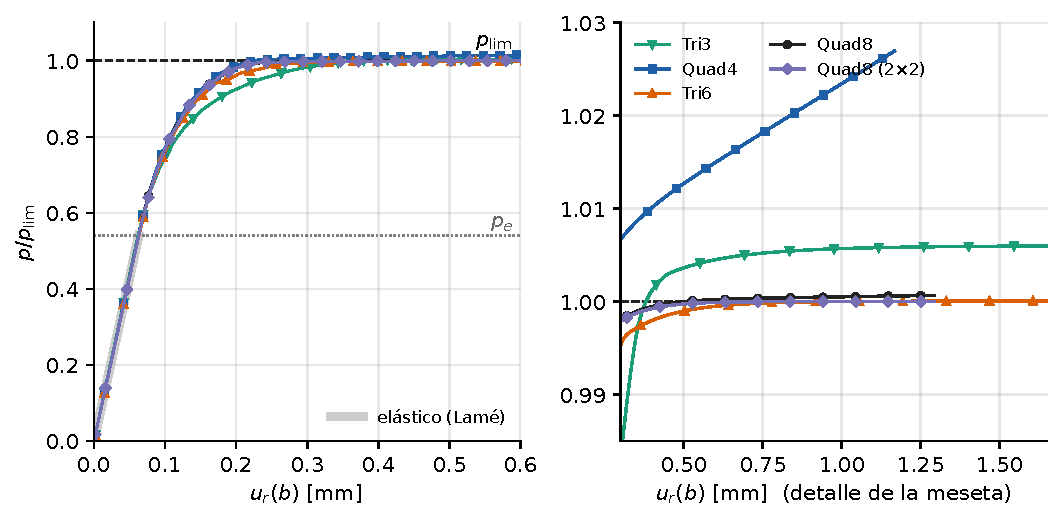
\includegraphics[width=0.9\linewidth]{../examples/cilindro_elastoplastico/fig_curvas.pdf}
\caption{Presión frente al desplazamiento radial exterior. Izquierda: curva completa. Derecha: detalle de la meseta de colapso, con la escala vertical ampliada.}
\label{fig:cilindro_elastoplastico:curvas}
\end{figure}

\begin{table}[h]
\centering
\caption{Cilindro elastoplástico. Error de la flexibilidad elástica frente a Lamé y carga relativa $p/p_{\mathrm{lim}}$ con desplazamientos exteriores de 0.5 y 1 mm.}
\begin{tabularx}{\textwidth}{YYYYY}
\hline
\textbf{Elemento} & \textbf{Grados de libertad} & \textbf{Error elástico} & \textbf{$p/p_{\mathrm{lim}}$ a 0.5 mm} & \textbf{$p/p_{\mathrm{lim}}$ a 1 mm} \\
\hline
Tri3, $8 \times 8$ & 162 & $1.8\times 10^{-2}$ & 1.0036 & 1.0057 \\
Quad4, $8 \times 8$ & 162 & $4.3\times 10^{-3}$ & 1.0127 & 1.0234 \\
Tri6, $4 \times 4$ & 162 & $3.0\times 10^{-5}$ & 0.9990 & 1.0000 \\
Quad8, $4 \times 4$ & 130 & $5.3\times 10^{-5}$ & 1.0000 & 1.0005 \\
Quad8 con 2\ensuremath{\times}2, $4 \times 4$ & 130 & $5.0\times 10^{-5}$ & 0.9997 & 1.0000 \\
\hline
\end{tabularx}
\end{table}
La \hyperref[fig:cilindro_elastoplastico:curvas]{figura~\ref*{fig:cilindro_elastoplastico:curvas}} y la tabla muestran tres tramos:

\begin{itemize}
  \item \textbf{Elástico.} Todas las curvas arrancan sobre la recta de Lamé. Los elementos cuadráticos reproducen su pendiente con un error del orden de $10^{-5}$; el Tri3, el más rígido, la sobrestima un $1.8\times 10^{-2}$.
  \item \textbf{Elastoplástico.} Las curvas se separan de la recta a partir de $p_e$, cuando la cara interior empieza a fluir, y se curvan a medida que la zona plástica avanza.
  \item \textbf{Colapso.} Tri6 y los dos Quad8 se aplanan sobre $p_{\mathrm{lim}}$: a 1 mm de desplazamiento la presión está a menos de $10^{-3}$ de la analítica. El Tri3 también forma una meseta, un $5.7\times 10^{-3}$ por encima. El Quad4 no la forma: gana un $1.1\times 10^{-2}$ de carga entre 0.5 y 1 mm, y sigue subiendo hasta el final del recorrido.
\end{itemize}

\section{Bloqueo volumétrico}

La deformación plástica no cambia el volumen. En el colapso, el mecanismo del tubo es un flujo radial isocórico, y el modelo sólo puede seguirlo si sus funciones de forma admiten un campo de desplazamiento sin cambio de volumen en los puntos de integración que fluyen. El Quad4 con integración completa impone esa condición en sus cuatro puntos de Gauss, más de las que su interpolación bilineal puede satisfacer, y el mecanismo discreto resulta más rígido que el real. Es el \textbf{bloqueo volumétrico}, descrito por Nagtegaal, Parks y Rice en 1974 precisamente para el régimen totalmente plástico.

El síntoma se ve en el esfuerzo medio, $(\sigma_{xx} + \sigma_{yy} + \sigma_{zz})/3$. En el colapso exacto vale $\sigma_{rr} + \sigma_y/\sqrt3$, entre $-54$ MPa en la cara interior y 139 MPa en la exterior. Con 1 mm de desplazamiento exterior, el Quad4 tiene puntos de Gauss entre $-223$ y 171 MPa: una presión espuria, que el criterio de von Mises no limita porque sólo acota la parte desviadora del esfuerzo. El Tri6 y los dos Quad8 quedan dentro del intervalo exacto, salvo el error de discretización.

El bloqueo no es un error del programa ni del material: el mapeo de retorno respeta la superficie de fluencia en todos los puntos y el equilibrio se cumple. Es una propiedad del elemento, y se evita eligiéndolo bien:

\begin{itemize}
  \item Los elementos cuadráticos, Tri6 y Quad8, no muestran bloqueo apreciable en este problema.
  \item El Quad8 con integración reducida 2\ensuremath{\times}2, que impone la condición en cuatro puntos en vez de nueve, da la meseta más plana. En el API se elige con el argumento \texttt{quadrature=\textquotedbl{}2x2\textquotedbl{}} del elemento, y en un YAML con elementos declarados uno a uno, con la clave \texttt{quadrature} de cada elemento.
  \item Solidum no tiene todavía formulaciones contra el bloqueo para el Quad4, como la B-barra o las mixtas desplazamiento-presión. Para plasticidad en deformación plana, o para materiales casi incompresibles, conviene usar elementos cuadráticos.
\end{itemize}

\section{Para seguir}

\begin{itemize}
  \item Añadir endurecimiento, \texttt{H \textgreater{} 0} en \texttt{VonMises2D}, y observar que la meseta se inclina: $p_{\mathrm{lim}}$ deja de ser una carga límite.
  \item Intentar superar $p_{\mathrm{lim}}$ con \texttt{NonlinearSolver} y control de carga. ¿Qué hace el solver cuando no hay equilibrio?
  \item Refinar la malla del Quad4. ¿Desaparece el bloqueo?
\end{itemize}

\textbf{Referencias.} R. Hill, \textit{The Mathematical Theory of Plasticity}, Oxford, 1950, cap. V. J. C. Nagtegaal, D. M. Parks y J. R. Rice, \textquotedbl{}On numerically accurate finite element solutions in the fully plastic range\textquotedbl{}, \textit{Computer Methods in Applied Mechanics and Engineering} 4 (1974) 153-177. E. A. de Souza Neto, D. Perić y D. R. J. Owen, \textit{Computational Methods for Plasticity}, Wiley, 2008, §7.5.

\textbf{Archivos del ejemplo.} La carpeta \texttt{examples/\allowbreak{}cilindro\_\allowbreak{}elastoplastico/\allowbreak{}} contiene el script \texttt{run.py}, que construye el modelo con las funciones del ejemplo 3, los resultados en \texttt{resultados.json} y la figura.


\newpage

\chapter{Barra con daño: localización, retroceso y control indirecto}
\chaptermark{Barra con daño}
\label{cap:barra_dano_localizado}





Una barra a tracción de un material que se ablanda: pasado el máximo, cuanto más se estira, menos fuerza soporta. Es el comportamiento del hormigón, de la roca o de la madera cuando se fisuran. El ejemplo muestra por qué ese tramo descendente no se puede recorrer controlando la carga, cómo el daño se concentra en una sola zona mientras el resto se descarga, y por qué una barra larga puede \textbf{retroceder}: desplazarse hacia atrás mientras la carga cae. Todo se compara con la solución exacta.

\textbf{Qué se aprende}

\begin{itemize}
  \item Usar un material de daño con ablandamiento (\texttt{IsotropicDamage1D}).
  \item Por qué el control de carga se detiene en el pico, y el de desplazamiento en un retroceso.
  \item Seguir el retroceso con \texttt{IndirectDisplacementSolver}, el \textbf{control indirecto de desplazamiento}.
  \item Que con ablandamiento un paso demasiado grande puede llevar a otro equilibrio.
\end{itemize}

\section{Planteamiento}

Una barra de sección $A =$ 100 cm\ensuremath{^{2}} empotrada en un extremo y cargada con una fuerza $F$ en el otro, dividida en elementos \texttt{Truss2D} de longitud $h =$ 0.1 m. El material tiene $E =$ 30 GPa y un daño isótropo que empieza cuando la deformación alcanza $\kappa_0 =$ $10^{-4}$, es decir, con un esfuerzo $\sigma_t = E\kappa_0 =$ 3.0 MPa. El elemento central es un 5 \% menos resistente: es la imperfección que decide dónde se localiza el daño, como en un ensayo real decide la zona más débil de la probeta.

Se estudian dos barras con el mismo tamaño de elemento: una \textbf{corta}, de 0.2 m (2 elementos), y una \textbf{larga}, de 1 m (10 elementos).

\section{Solución analítica}

\textbf{El material.} Con la variable de historia $\kappa$, la deformación máxima alcanzada, el daño y el esfuerzo son

\[
d(\kappa) = 1 - \frac{\kappa_0}{\kappa}\,e^{-\alpha(\kappa - \kappa_0)} \quad (\kappa > \kappa_0),
\qquad
\sigma = (1 - d)\,E\,\varepsilon ,
\]

con $\alpha =$ 5000. En carga, $\sigma = E\kappa_0\,e^{-\alpha(\varepsilon - \kappa_0)}$: el esfuerzo cae exponencialmente desde $\sigma_t$. En descarga, el material vuelve al origen por la secante, sin más daño.

\textbf{Localización.} Sin fuerzas de volumen, el equilibrio impone el mismo esfuerzo en toda la barra. La carga máxima la fija el elemento débil, $F_{\mathrm{pico}} = A\,E\,\kappa_{0w} =$ 28.5 kN, con $\kappa_{0w}$ su umbral. Pasado el pico el esfuerzo baja; el elemento débil sigue dañándose, pero los demás, que nunca llegaron a su umbral, se descargan elásticamente. Con la deformación del elemento débil $\varepsilon_w$ como parámetro, la respuesta exacta es

\[
F = A\,\sigma(\varepsilon_w),
\qquad
u = h\,\varepsilon_w + (L - h)\,\frac{\sigma(\varepsilon_w)}{E} .
\]

\textbf{Retroceso.} Justo después del pico, $d\sigma/d\varepsilon_w = -\alpha\,\sigma$, y el desplazamiento del extremo cambia a razón de

\[
\frac{du}{d\varepsilon_w} = h - (L - h)\,\alpha\,\kappa_{0w} .
\]

Si es negativa, el desplazamiento \textbf{disminuye} mientras la carga cae: la curva retrocede (\textit{snap-back}). Ocurre cuando $(L/h - 1)\,\alpha\,\kappa_{0w} > 1$. Ese producto vale 0.475 en la barra corta y 4.275 en la larga: la corta baja sin más; la larga retrocede hasta $u =$ 0.616 $u_{\mathrm{pico}}$ antes de volver a avanzar.

El balance de energía lo explica. El elemento débil disipa en toda su rotura 0.705 J, lo mismo en las dos barras porque tiene el mismo tamaño. En el pico, la barra corta tiene almacenados 0.271 J de energía elástica y la larga 1.354 J. Al romperse, toda esa energía elástica se libera, y la parte que el elemento no puede disipar tiene que devolverse a la carga exterior. Para eso el trabajo de la fuerza tiene que ser negativo, y con la fuerza a tracción eso sólo ocurre si el extremo retrocede. La barra corta no tiene exceso que devolver.

\section{Modelo en Solidum}

La barra se construye elemento a elemento, con el central debilitado:

\begin{lstlisting}[language=Python]
def barra(L: float):
    """Barra de ``L/H`` elementos ``Truss2D`` con el central debilitado,
    empotrada en ``x = 0``. Devuelve el dominio, el nodo del extremo libre y
    el elemento débil; cada control añade su carga o su apoyo."""
    n = round(L / H)
    dom = Domain()
    nodos = [dom.add_node(i + 1, [i * H, 0.0]) for i in range(n + 1)]
    for k in range(n):
        umbral = K0W if k == n // 2 else KAPPA_0
        material = IsotropicDamage1D(E=E, kappa_0=umbral, alpha=ALPHA)
        dom.add_element(Truss2D(k + 1, [nodos[k], nodos[k + 1]], material, A=A))
    nodos[0].fix_dof("ux", 0.0)
    for nodo in nodos:
        nodo.fix_dof("uy", 0.0)
    extremo, debil = nodos[-1], dom.elements[n // 2 + 1]
    return dom, extremo, debil

\end{lstlisting}

Se resuelve con tres controles distintos:

\begin{itemize}
  \item \textbf{Control de carga} (\href{https://github.com/jretamav/solidum-fem/blob/main/docs/specs/NonlinearSolver.md}{NonlinearSolver} con una fuerza creciente hasta 1.2 veces la de pico). Impone la carga de cada paso, y por encima de $F_{\mathrm{pico}}$ no hay equilibrio.
  \item \textbf{Control de desplazamiento} (el mismo solver con el desplazamiento del extremo impuesto). La carga es ahora la reacción, y puede bajar; pero el desplazamiento impuesto sólo crece.
  \item \textbf{Control indirecto} (\href{https://github.com/jretamav/solidum-fem/blob/main/docs/specs/IndirectDisplacementSolver.md}{IndirectDisplacementSolver}). Hace crecer en cada paso una magnitud elegida, aquí el alargamiento del elemento débil, y deja libres a la vez la carga y el desplazamiento del extremo. Es como se controla en laboratorio un ensayo de fractura, con la apertura de la fisura:
\end{itemize}

\begin{lstlisting}[language=Python]
def control_indirecto(L: float, dlambda: float = DLAMBDA, pasos: int = 500):
    """Control indirecto sobre el alargamiento del elemento débil."""
    dom, extremo, debil = barra(L)
    dom.generate_equation_numbers(verbose=False)
    F = np.zeros(dom.total_dofs)
    F[extremo.dofs["ux"]] = F_PICO
    a, b = debil.nodes
    solver = IndirectDisplacementSolver(
        Assembler(dom), control=[(b, "ux", 1.0), (a, "ux", -1.0)],
        initial_dlambda=dlambda, max_lambda=1.2, max_steps=pasos, max_iter=30)
    curva: list = []
    solver.solve(F, step_callback=_registro(dom, extremo, debil, curva,
                                            lambda U, lam: lam * F_PICO))
    return np.array(curva)

\end{lstlisting}

La magnitud controlada se declara como una combinación de grados de libertad, $\mathbf c^\top\mathbf U$: aquí, $u_b - u_a$ entre los dos nodos del elemento débil. El primer paso es un 2 \% de la carga de pico, y el solver mantiene constante ese incremento de alargamiento en todo el trazado.

\section{Resultados}

\begin{figure}[H]
\centering
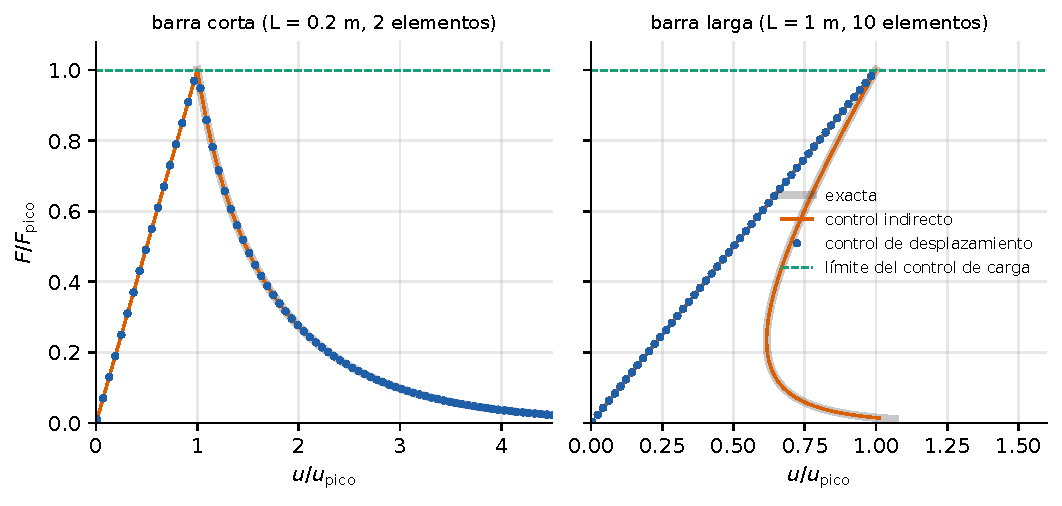
\includegraphics[width=0.9\linewidth]{../examples/barra_dano_localizado/fig_curvas.pdf}
\caption{Carga frente al desplazamiento del extremo, normalizados con el pico. La curva exacta en gris.}
\label{fig:barra_dano_localizado:curvas}
\end{figure}

\begin{table}[h]
\centering
\caption{Qué consigue cada control en cada barra. El error se mide frente a la solución exacta con la misma deformación del elemento débil.}
\begin{tabularx}{\textwidth}{YYY}
\hline
\textbf{Control} & \textbf{Barra corta} & \textbf{Barra larga} \\
\hline
Carga & se detiene en el pico & se detiene en el pico \\
Desplazamiento del extremo & curva completa, error menor que $10^{-12}$ & se detiene en el pico, $u =$ 1.000 $u_{\mathrm{pico}}$ \\
Indirecto & curva completa, error menor que $10^{-12}$ & curva completa, error menor que $10^{-12}$; retrocede hasta 0.616 $u_{\mathrm{pico}}$ \\
\hline
\end{tabularx}
\end{table}
La \hyperref[fig:barra_dano_localizado:curvas]{figura~\ref*{fig:barra_dano_localizado:curvas}} resume los tres comportamientos:

\begin{itemize}
  \item \textbf{El control de carga} llega hasta $F_{\mathrm{pico}}$ en las dos barras y ahí termina con un error de divergencia (\texttt{UnknownDivergenceError}): el solver reduce el paso sin encontrar equilibrio por encima.
  \item \textbf{El control de desplazamiento} recorre toda la rama descendente de la barra corta, sobre la curva exacta. En la larga se detiene en el pico: a partir de ahí el camino de equilibrio sigue con desplazamientos \textit{menores}. Con un desplazamiento impuesto mayor que el del pico, el único equilibrio que queda en el camino físico está al otro lado del lazo, con la carga casi nula, y el solver no llega a él.
  \item \textbf{El control indirecto} sigue las dos curvas exactas, incluido el retroceso de la larga, con un solo elemento dañado en todo el trazado. En las dos barras llega a una carga de 0.014 veces la de pico en 500 pasos.
\end{itemize}

El arco cilíndrico de \href{https://github.com/jretamav/solidum-fem/blob/main/docs/specs/ArcLengthSolver.md}{ArcLengthSolver}, con el mismo primer paso, tampoco sigue el retroceso: en la barra larga termina en el pico con un error (\texttt{RuntimeError}) sin haber retrocedido. Tras el pico, la parte de la barra que se descarga invierte casi por completo el sentido de su desplazamiento, y el criterio con que ese solver elige la solución, la más alineada con el paso anterior, la descarta.

\begin{warnbox}{Advertencia}
Con ablandamiento, el problema de cada paso puede tener más de una solución. Además de la física, en la que sólo se daña el elemento débil, hay otras en las que también se dañan elementos que en realidad se habrían descargado. Cuál encuentra el solver depende de su punto de partida. Si un paso sobrepasa el pico más que la imperfección que localiza el daño, aquí un 5 \%, el solver puede converger a otra. Con pasos del 10 \% de la carga, el control indirecto de la barra larga acaba con los 10 elementos dañados y un desplazamiento que se aparta hasta 9 veces $u_{\mathrm{pico}}$ de la solución exacta (\hyperref[fig:barra_dano_localizado:salto]{figura~\ref*{fig:barra_dano_localizado:salto}}). No es propio de este solver: el control de desplazamiento de la barra corta con 12 pasos termina con sus 2 elementos dañados. La defensa es un paso pequeño cerca del pico; por eso \texttt{IndirectDisplacementSolver} no agranda el paso por omisión.
\end{warnbox}

\begin{figure}[H]
\centering
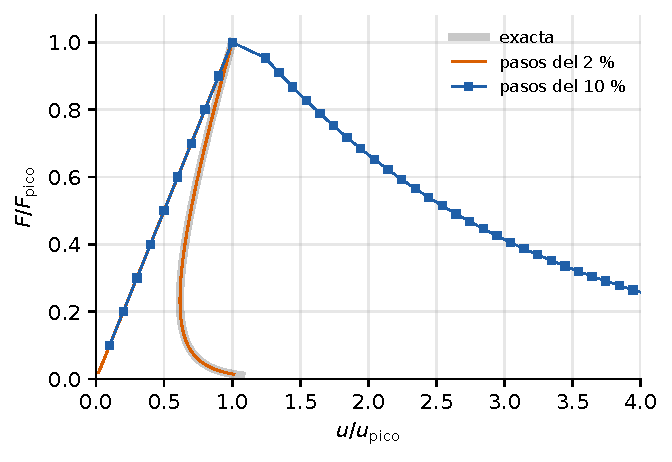
\includegraphics[width=0.9\linewidth]{../examples/barra_dano_localizado/fig_salto.pdf}
\caption{Barra larga con control indirecto: con pasos del 2 \% se sigue la curva exacta; con pasos del 10 \% el solver salta a otro equilibrio, con todos los elementos dañados.}
\label{fig:barra_dano_localizado:salto}
\end{figure}

\section{Para seguir}

\begin{itemize}
  \item Refinar la malla de la barra larga, con $h$ más pequeño. ¿Qué pasa con el retroceso? Con daño local la zona que se rompe mide siempre un elemento, y la energía disipada es proporcional a $h$: el resultado depende de la malla. Los modelos regularizados, o los de fisura cohesiva, que disipan una energía de fractura por unidad de área, corrigen esa dependencia.
  \item Reducir la imperfección del elemento débil al 1 \% y repetir la advertencia. ¿Qué paso hace falta ahora?
  \item Controlar con el control indirecto el desplazamiento del extremo en vez del alargamiento del elemento débil. ¿Hasta dónde llega en la barra larga?
\end{itemize}

\textbf{Referencias.} R. de Borst, \textquotedbl{}Computation of post-bifurcation and post-failure behavior of strain-softening solids\textquotedbl{}, \textit{Computers \& Structures} 25 (1987) 211-224. M. A. Crisfield, \textit{Non-linear Finite Element Analysis of Solids and Structures}, vol. 1, Wiley, 1991, cap. 9. Z. P. Bažant y J. Planas, \textit{Fracture and Size Effect in Concrete and Other Quasibrittle Materials}, CRC Press, 1998.

\textbf{Archivos del ejemplo.} La carpeta \texttt{examples/\allowbreak{}barra\_\allowbreak{}dano\_\allowbreak{}localizado/\allowbreak{}} contiene el script \texttt{run.py}, los resultados en \texttt{resultados.json} y las dos figuras.


\newpage

\chapter{Flexión pura de un prisma: el bloqueo por cortante del Hex8}
\chaptermark{Flexión pura de un prisma}
\label{cap:flexion_pura_3d}





El estado de flexión más simple, un prisma sometido a un momento constante, tiene solución exacta de la elasticidad tridimensional. Es una prueba exigente para un elemento sólido: debe representar a la vez la flexión y la deformación de la sección por el efecto de Poisson. El Hex20 la reproduce exactamente con un solo elemento. El Hex8 no: se vuelve demasiado rígido por una distorsión angular que la flexión pura no tiene. Es el \textbf{bloqueo por cortante}, el segundo tipo de bloqueo del manual después del volumétrico del ejemplo 4.

\textbf{Qué se aprende}

\begin{itemize}
  \item Construir desde el API una malla estructurada de \texttt{Hex8} o \texttt{Hex20}.
  \item Imponer una curvatura con desplazamientos y medir el momento de reacción.
  \item Reconocer y cuantificar el bloqueo por cortante.
  \item Elegir el elemento en problemas dominados por la flexión.
\end{itemize}

\section{Planteamiento}

Un prisma de acero de longitud $L =$ 1 m y sección cuadrada de lado $h =$ 10 cm, con $E =$ 200 GPa y $\nu =$ 0.3, se flexiona en el plano $xz$ con una curvatura uniforme $\kappa =$ 0.01 $\mathrm{m}^{-1}$. El esfuerzo máximo es $\sigma_{\max} = E\kappa h/2 =$ 100 MPa.

\section{Solución analítica}

En flexión pura la única componente del esfuerzo es $\sigma_{xx} = E\,\kappa\,z$; con la convención del proyecto, una curvatura positiva tracciona las fibras con $z > 0$ y equivale a un momento $M_y = E\kappa I =$ 16.667 kN\ensuremath{\cdot}m, con $I = h^4/12$. Integrando las deformaciones se obtiene el desplazamiento exacto (Saint-Venant):

\[
u = \kappa\,x\,z,
\qquad
v = -\nu\,\kappa\,y\,z,
\qquad
w = -\frac{\kappa\,x^2}{2} + \frac{\nu\,\kappa}{2}\,(y^2 - z^2).
\]

Las secciones permanecen planas ($u$ es lineal en $z$), pero no conservan su forma: por el efecto de Poisson, las fibras traccionadas se estrechan y las comprimidas se ensanchan, y la sección se curva en sentido contrario al eje. Es la \textbf{curvatura anticlástica}, el término $\nu$ de $v$ y $w$. El desplazamiento es un polinomio de segundo grado en $x$, $y$, $z$.

\section{Modelo en Solidum}

La malla se construye elemento a elemento sobre una rejilla de nodos; el \texttt{Hex20} usa los vértices y los medios de arista. Las condiciones de contorno reproducen la solución exacta sin añadir restricciones que ella no cumpla:

\begin{lstlisting}[language=Python]
def resolver(elemento: str, nx: int, n: int, nu: float = NU) -> dict:
    """Curvatura impuesta con ``u`` en los extremos; sólido rígido fijado en
    dos esquinas de la raíz con los valores exactos."""
    dom, nodos, q = malla(elemento, nx, n, nu)
    extremo = []
    for nodo in dom.nodes.values():
        x, y, z = nodo.coordinates
        if abs(x) < 1e-12:
            nodo.fix_dof("ux", 0.0)
        elif abs(x - L) < 1e-12:
            nodo.fix_dof("ux", KAPPA * L * z)
            extremo.append(nodo)
    esquina_a, esquina_b = nodos[(0, 0, 0)], nodos[(0, q * n, 0)]
    esquina_a.fix_dof("uy", exacta(*esquina_a.coordinates, nu)[1])
    esquina_a.fix_dof("uz", exacta(*esquina_a.coordinates, nu)[2])
    esquina_b.fix_dof("uz", exacta(*esquina_b.coordinates, nu)[2])

    dom.generate_equation_numbers(verbose=False)
    asm = Assembler(dom)
    U = LinearSolver(asm).solve(np.zeros(dom.total_dofs))
    _, F_int = asm.assemble_non_linear_system(U)
    # Momento de reacción en el extremo: Σ R_x·z (R = fuerza interna nodal).
    M = sum(F_int[nodo.dofs["ux"]] * nodo.coordinates[2] for nodo in extremo)

    error_u = max(abs(U[nodo.dofs[d]] - exacta(*nodo.coordinates, nu)[k])
                  for nodo in dom.nodes.values() for k, d in enumerate(("ux", "uy", "uz")))
    sxz = 0.0
    for el in dom.elements.values():
        estado = el.compute_gauss_state(U)
        sxz = max(sxz, float(np.max(np.abs(np.asarray(estado["stress"])[:, 5]))))
    a = L / nx                                    # longitud del elemento
    g = E / (2 * (1 + nu))
    sxz_teorico = g * KAPPA * a / (2 * np.sqrt(3)) if elemento == "Hex8" else 0.0
    # Energía del cortante parásito frente a la de flexión: (a/h)²/(2(1+ν)).
    cortante = (a / B) ** 2 / (2 * (1 + nu)) if elemento == "Hex8" else 0.0
    return {"elemento": elemento, "nx": nx, "n": n, "gdl": int(dom.total_dofs),
            "a_sobre_h": a / B, "M_sobre_exacto": M / (E * KAPPA * I),
            "exceso_cortante": cortante,
            "exceso_resto": M / (E * KAPPA * I) - 1 - cortante,
            "error_M": abs(M / (E * KAPPA * I) - 1),
            "error_M_pct": 100 * abs(M / (E * KAPPA * I) - 1),
            "error_u": error_u / (KAPPA * L * L / 2),
            "sxz_sobre_smax": sxz / SIGMA_MAX,
            "sxz_teorico_sobre_smax": sxz_teorico / SIGMA_MAX,
            "error_sxz_teorico": abs(sxz - sxz_teorico) / SIGMA_MAX}

\end{lstlisting}

\begin{itemize}
  \item En los dos extremos se impone el desplazamiento axial exacto: $u = 0$ en $x = 0$ y $u = \kappa L z$ en $x = L$. Es la curvatura impuesta.
  \item Los movimientos de sólido rígido que quedan libres (dos traslaciones y el giro alrededor del eje) se fijan en dos esquinas de la sección de la raíz, con los valores exactos. No se empotra la raíz: el empotramiento impediría la curvatura anticlástica y el estado dejaría de ser flexión pura.
  \item El momento se mide como la reacción del extremo, $M = \sum R_x\,z$ sobre sus nodos.
\end{itemize}

\section{Resultados}

\begin{figure}[H]
\centering
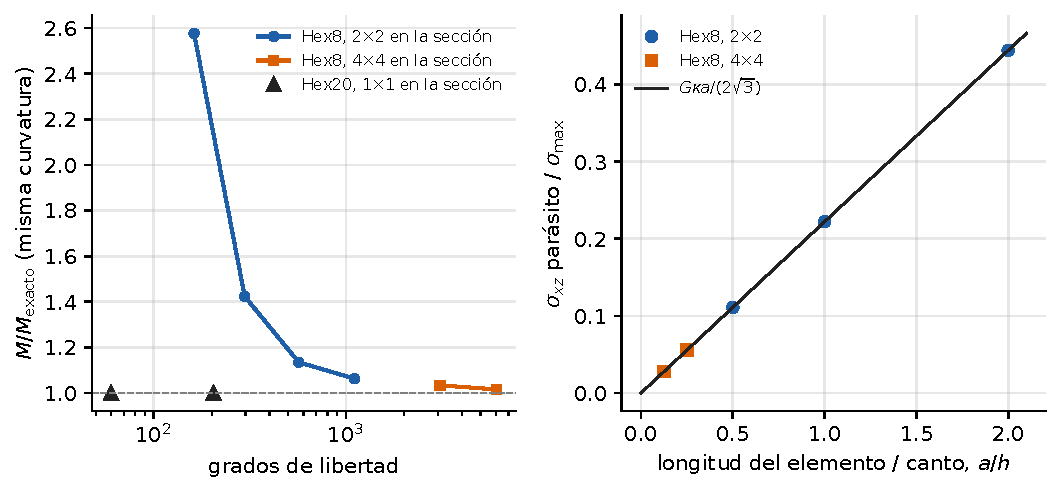
\includegraphics[width=0.9\linewidth]{../examples/flexion_pura_3d/fig_bloqueo.pdf}
\caption{Izquierda: momento necesario para la misma curvatura, relativo al exacto, frente al número de grados de libertad. Derecha: esfuerzo cortante parásito en los puntos de Gauss del Hex8 frente a la longitud del elemento; la recta es la fórmula del texto.}
\label{fig:flexion_pura_3d:bloqueo}
\end{figure}

\begin{table}[h]
\centering
\caption{Momento necesario para imponer la curvatura, relativo al exacto, y esfuerzo cortante parásito en los puntos de Gauss. $a$ es la longitud del elemento.}
\begin{tabularx}{\textwidth}{YYYYYY}
\hline
\textbf{Elemento} & \textbf{Malla} & \textbf{Grados de libertad} & \textbf{$a/h$} & \textbf{$M/M_{\mathrm{exacto}}$} & \textbf{$\sigma_{xz}/\sigma_{\max}$} \\
\hline
Hex8 & $5 \times 2 \times 2$ & 162 & 2.000 & 2.5772 & 0.444 \\
Hex8 & $10 \times 2 \times 2$ & 297 & 1.000 & 1.4234 & 0.222 \\
Hex8 & $20 \times 2 \times 2$ & 567 & 0.500 & 1.1349 & 0.111 \\
Hex8 & $40 \times 2 \times 2$ & 1107 & 0.250 & 1.0628 & 0.056 \\
Hex8 & $40 \times 4 \times 4$ & 3075 & 0.250 & 1.0338 & 0.056 \\
Hex8 & $80 \times 4 \times 4$ & 6075 & 0.125 & 1.0157 & 0.028 \\
Hex20 & $1 \times 1 \times 1$ & 60 & 10.000 & 1.0000 & 0 \\
Hex20 & $5 \times 1 \times 1$ & 204 & 2.000 & 1.0000 & 0 \\
\hline
\end{tabularx}
\end{table}
\textbf{El Hex20 es exacto.} Con un solo elemento, 60 grados de libertad, reproduce el momento, los desplazamientos y los esfuerzos de la solución exacta con un error menor que $10^{-10}$, y su esfuerzo cortante es nulo. No es casualidad: sus funciones de forma contienen todos los polinomios de segundo grado, y la solución exacta es uno de ellos.

\textbf{El Hex8 es demasiado rígido.} Para imponer la misma curvatura necesita 2.58 veces el momento exacto en la malla más gruesa, y todavía un 1.6 \% más con 6075 grados de libertad, cien veces más que el Hex20. Los desplazamientos, impuestos a través de la curvatura, salen casi exactos: el error está en la rigidez. Si la carga fuera una fuerza, ese exceso de rigidez daría desplazamientos menores que los reales.

\section{El bloqueo por cortante}

Dentro de un Hex8 los desplazamientos son lineales en cada dirección, así que la flecha $w$ de cada elemento es lineal en $x$: el elemento no puede curvarse, sólo girar. El giro de la sección, $\partial u/\partial z = \kappa x$, crece en cambio a lo largo del elemento. La diferencia entre ambos es una distorsión angular que la flexión pura no tiene,

\[
\gamma_{xz} = \frac{\partial u}{\partial z} + \frac{\partial w}{\partial x} = \kappa\,(x - x_c),
\]

con $x_c$ el centro del elemento. En los puntos de Gauss, $x - x_c = \pm a/(2\sqrt3)$, y aparece un esfuerzo cortante \textbf{parásito}

\[
\sigma_{xz} = \frac{G\,\kappa\,a}{2\sqrt3},
\qquad
\frac{\sigma_{xz}}{\sigma_{\max}} = \frac{a/h}{2\sqrt3\,(1+\nu)} = 0.222\,\frac{a}{h} .
\]

La \hyperref[fig:flexion_pura_3d:bloqueo]{figura~\ref*{fig:flexion_pura_3d:bloqueo}} lo confirma: los valores calculados caen sobre la recta, y sólo dependen de la longitud del elemento, no de cuántos elementos haya en la sección. La energía de ese cortante se suma a la de flexión y hace al elemento más rígido. Su cociente con la energía de flexión da el exceso de momento:

\[
\frac{M}{M_{\mathrm{exacto}}} - 1 \approx \frac{(a/h)^2}{2(1+\nu)} .
\]

Con $a/h =$ 2 son 1.538 de los 1.577 medidos. El resto, 0.039 con dos elementos por lado de la sección y 0.010 con cuatro, no depende de $a$: es la sección, que con elementos lineales no representa la curvatura anticlástica, cuadrática en $y$, $z$. La prueba es que con $\nu = 0$, sin curvatura anticlástica, la malla de $5 \times 2 \times 2$ da exactamente $M/M_{\mathrm{exacto}} =$ 3.0000 $= 1 + (a/h)^2/2$.

El error por cortante decrece como $(a/h)^2$: se reduce refinando \textbf{a lo largo} del prisma, y lentamente. La solución práctica es cambiar de elemento:

\begin{itemize}
  \item Los elementos cuadráticos, Hex20 y Hex27, representan la flexión sin distorsión parásita.
  \item Existen formulaciones del Hex8 que eliminan el bloqueo: modos incompatibles, deformaciones mejoradas o integración reducida con control de los modos espurios. Solidum no las tiene todavía. El Hex8 admite integración reducida (\texttt{quadrature=\textquotedbl{}hex\_\allowbreak{}1x1x1\textquotedbl{}}), pero sin ese control es propenso a modos de energía nula (\textit{hourglass}). En problemas dominados por la flexión conviene usar el Hex20.
\end{itemize}

Es el mismo fenómeno que el bloqueo volumétrico del ejemplo 4: el elemento lineal impone en sus puntos de integración una condición que su cinemática no puede cumplir, allí la de no cambiar de volumen y aquí la de no distorsionarse, y responde con una rigidez espuria.

\section{Para seguir}

\begin{itemize}
  \item Distorsionar la malla del Hex20, moviendo los nodos interiores. ¿Sigue siendo exacto? Su exactitud depende de que la geometría de cada elemento sea un paralelepípedo.
  \item Cargar el prisma en voladizo con una fuerza en el extremo y comparar la flecha del Hex8 y del Hex20 con la de la teoría de vigas.
  \item Repetir con el \texttt{Hex27}.
\end{itemize}

\textbf{Referencias.} S. P. Timoshenko y J. N. Goodier, \textit{Theory of Elasticity}, 3.ª ed., McGraw-Hill, 1970 (flexión pura de barras prismáticas). R. H. MacNeal y R. L. Harder, \textquotedbl{}A proposed standard set of problems to test finite element accuracy\textquotedbl{}, \textit{Finite Elements in Analysis and Design} 1 (1985) 3-20. R. D. Cook, D. S. Malkus, M. E. Plesha y R. J. Witt, \textit{Concepts and Applications of Finite Element Analysis}, 4.ª ed., Wiley, 2002.

\textbf{Archivos del ejemplo.} La carpeta \texttt{examples/\allowbreak{}flexion\_\allowbreak{}pura\_\allowbreak{}3d/\allowbreak{}} contiene el script \texttt{run.py}, los resultados en \texttt{resultados.json} y la figura.


\newpage

\chapter{Edificio de cinco niveles: análisis modal y espectro de respuesta}
\chaptermark{Edificio de cinco niveles}
\label{cap:edificio_espectro}





El análisis sísmico por espectro de respuesta es la herramienta de diseño habitual de la ingeniería de edificios: se calculan los modos de vibrar de la estructura, se lee en el espectro la respuesta máxima de cada uno y se combinan. Este ejemplo lo hace sobre un marco de cinco niveles cuya versión idealizada, el edificio de cortante, tiene solución cerrada, y repite la combinación a mano con los modos analíticos para comprobar cada paso.

\textbf{Qué se aprende}

\begin{itemize}
  \item Modelar un marco con \texttt{Frame2DEuler}, con la masa concentrada en las losas.
  \item Calcular frecuencias y modos con \texttt{ModalSolver}.
  \item Hacer un análisis espectral con \texttt{ResponseSpectrumSolver}: masas efectivas, combinación SRSS y CQC.
  \item Combinar correctamente las respuestas: las derivas de entrepiso se combinan modo a modo.
\end{itemize}

\section{Planteamiento}

Un marco de concreto de 5 niveles y un vano, con entrepisos de $h =$ 3 m y claro de 6 m. Las columnas son de 40 \ensuremath{\times} 40 cm, con $E =$ 25 GPa, y cada nivel tiene una masa $m =$ 30 t.

Se adoptan las hipótesis del \textbf{edificio de cortante}: losas infinitamente rígidas y columnas inextensibles. En el modelo, las losas son vigas con una rigidez a flexión $10^{4}$ veces la de una columna, las columnas tienen un área $10^{4}$ veces la real, y toda la masa está en las losas. Así cada columna trabaja biempotrada, y la rigidez lateral de cada entrepiso es

\[
k = 2\,\frac{12\,E\,I}{h^3} = \text{ 47.4 MN/m} .
\]

El sismo se representa con un espectro de diseño simplificado de aceleración, para un amortiguamiento del 5 \%: una rampa desde la aceleración del terreno $a_0 =$ 0.30 $g$ hasta una meseta de $2.5\,a_0$ entre $T_B =$ 0.1 s y $T_C =$ 0.5 s, y una caída proporcional a $1/T$ después.

\section{Solución analítica}

El edificio de cortante es una cadena de masas $m$ y resortes $k$ iguales, empotrada en la base. Sus frecuencias y modos tienen expresión cerrada:

\[
\omega_j = 2\sqrt{\frac{k}{m}}\,\sin\frac{(2j-1)\,\pi}{2(2n+1)},
\qquad
\phi_j(i) = \sin\frac{(2j-1)\,i\,\pi}{2n+1},
\qquad i, j = 1, \dots, n .
\]

Con ellos se calculan a mano, sin Solidum, el factor de participación y la masa efectiva de cada modo,

\[
\Gamma_j = \frac{\sum_i m\,\phi_j(i)}{\sum_i m\,\phi_j(i)^2},
\qquad
M_j^* = \frac{\left(\sum_i m\,\phi_j(i)\right)^2}{\sum_i m\,\phi_j(i)^2},
\]

el desplazamiento máximo de cada modo, $u_j(i) = \Gamma_j\,\phi_j(i)\,S_a(T_j)/\omega_j^2$, y el cortante basal modal, $V_j = M_j^*\,S_a(T_j)$. La combinación SRSS toma la raíz de la suma de los cuadrados de las respuestas modales.

\section{Modelo en Solidum}

El marco se construye con dos columnas y una losa por nivel. Las columnas usan un material con densidad nula; la densidad de la losa se elige para que su masa sea la del piso:

\begin{lstlisting}[language=Python]
def marco(rigidez: float = RIGIDEZ):
    """Marco de ``N`` niveles y un vano. Columnas ``Frame2DEuler`` sin masa;
    cada losa es una viga ``rigidez`` veces más rígida que una columna, con
    la masa del piso. Las columnas tienen área ``rigidez`` veces la real
    (inextensibles). Devuelve el dominio y los nodos por ``(nivel, lado)``."""
    dom = Domain()
    columna = Elastic1D(E=E, density=0.0)
    A_losa = rigidez * A_COL
    losa = Elastic1D(E=E, density=M_PISO / (A_losa * CLARO))
    nodos = {}
    for i in range(N + 1):
        for lado, x in enumerate((0.0, CLARO)):
            nodos[(i, lado)] = dom.add_node(len(nodos) + 1, [x, i * H])
    for i in range(N):
        for lado in (0, 1):
            dom.add_element(Frame2DEuler(len(dom.elements) + 1,
                                         [nodos[(i, lado)], nodos[(i + 1, lado)]],
                                         columna, A=rigidez * A_COL, I=I_COL))
        dom.add_element(Frame2DEuler(len(dom.elements) + 1,
                                     [nodos[(i + 1, 0)], nodos[(i + 1, 1)]],
                                     losa, A=A_losa, I=rigidez * I_COL))
    for lado in (0, 1):
        for dof in ("ux", "uy", "rz"):
            nodos[(0, lado)].fix_dof(dof, 0.0)
    dom.generate_equation_numbers(verbose=False)
    return dom, nodos

\end{lstlisting}

El análisis espectral calcula internamente los modos, los combina y devuelve la respuesta máxima:

\begin{lstlisting}[language=Python]
def espectral(combinacion: str = "SRSS"):
    """Análisis espectral con Solidum; devuelve el resultado y los nodos."""
    dom, nodos = marco()
    solver = ResponseSpectrumSolver(
        Assembler(dom), n_modes=N, direction={"dof_name": "ux"},
        spectrum=lambda w: Sa(2 * np.pi / w) / w**2,       # S_d = S_a/ω²
        combination=combinacion, damping=0.05)
    return solver.solve(), nodos

\end{lstlisting}

La dirección del sismo se declara por el nombre del grado de libertad (\texttt{ux} en todos los nodos), y el espectro como una función de la frecuencia que devuelve el desplazamiento espectral, $S_d = S_a/\omega^2$. También se puede dar como tabla de periodos y valores, que es lo habitual desde el YAML.

\section{Resultados}

\begin{figure}[H]
\centering
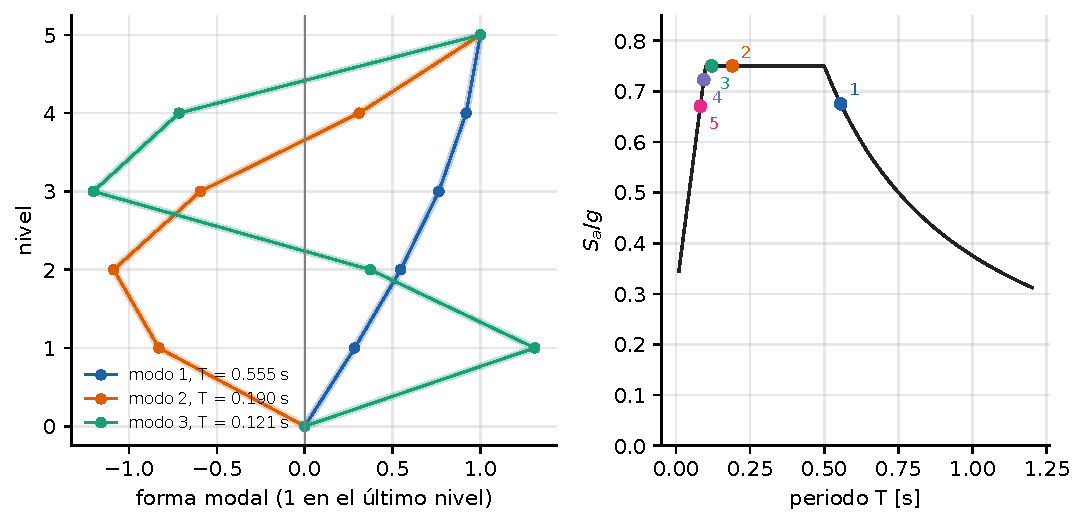
\includegraphics[width=0.9\linewidth]{../examples/edificio_espectro/fig_modos.pdf}
\caption{Izquierda: los tres primeros modos, Solidum (puntos) sobre los analíticos (bandas). Derecha: el espectro de diseño con los periodos de los cinco modos.}
\label{fig:edificio_espectro:modos}
\end{figure}

\begin{table}[h]
\centering
\caption{Periodos, masas efectivas y aceleración espectral de cada modo.}
\begin{tabularx}{\textwidth}{YYYYYY}
\hline
\textbf{Modo} & \textbf{$T$ exacto [s]} & \textbf{$T$ Solidum [s]} & \textbf{Masa efectiva} & \textbf{Acumulada} & \textbf{$S_a/g$} \\
\hline
1 & 0.5553 & 0.5554 & 88.0 \% & 88.0 \% & 0.675 \\
2 & 0.1902 & 0.1903 & 8.7 \% & 96.7 \% & 0.750 \\
3 & 0.1207 & 0.1207 & 2.4 \% & 99.1 \% & 0.750 \\
4 & 0.0939 & 0.0939 & 0.8 \% & 99.8 \% & 0.723 \\
5 & 0.0824 & 0.0824 & 0.2 \% & 100.0 \% & 0.671 \\
\hline
\end{tabularx}
\end{table}
\textbf{Modos.} Los periodos coinciden con los de la solución cerrada con una diferencia relativa de $1.7\times 10^{-4}$, y las formas modales con $3\times 10^{-4}$. Esa pequeña diferencia es la rigidez finita de losas y columnas: con las losas diez veces más rígidas baja a $1.7\times 10^{-5}$. El edificio de cortante es el límite del marco cuando las losas se vuelven rígidas. El primer modo concentra el 88 \% de la masa; con tres modos se supera el 99 \%. Los reglamentos piden incluir modos hasta reunir al menos el 90 \%.

\begin{table}[h]
\centering
\caption{Desplazamiento máximo de cada nivel con SRSS y deriva de entrepiso combinada de dos maneras.}
\begin{tabularx}{\textwidth}{YYYYY}
\hline
\textbf{Nivel} & \textbf{$u$ Solidum [mm]} & \textbf{$u$ a mano [mm]} & \textbf{Deriva, modo a modo [mm]} & \textbf{Deriva, restando desplazamientos [mm]} \\
\hline
1 & 18.56 & 18.56 & 18.56 & 18.56 \\
2 & 35.48 & 35.48 & 16.97 & 16.93 \\
3 & 49.49 & 49.48 & 14.15 & 14.00 \\
4 & 59.54 & 59.53 & 10.32 & 10.05 \\
5 & 64.83 & 64.82 & 5.57 & 5.29 \\
\hline
\end{tabularx}
\end{table}
\textbf{Respuesta espectral.} Los desplazamientos SRSS de Solidum coinciden con los combinados a mano con los modos analíticos a $1.7\times 10^{-4}$. El cortante basal, combinando los cortantes modales, vale 879.5 kN (879.7 kN a mano): 0.598 veces el peso del edificio.

\textbf{SRSS y CQC.} La combinación cuadrática completa (CQC) tiene en cuenta la correlación entre modos de frecuencias cercanas. Aquí los modos están bien separados y los desplazamientos CQC quedan entre 0.9997 y 1.0011 veces los SRSS. La diferencia importa cuando hay modos próximos, por ejemplo en edificios con torsión.

\begin{warnbox}{Advertencia}
Las respuestas máximas de los modos no ocurren a la vez y la combinación pierde su signo, así que \textbf{cada magnitud de diseño se combina por separado}. La deriva de un entrepiso se calcula en cada modo y después se combina; restar los desplazamientos ya combinados de dos niveles consecutivos da otro valor. En este edificio subestima la deriva del último entrepiso: 5.29 mm en lugar de 5.57 mm. Lo mismo vale para los esfuerzos y las fuerzas internas de los elementos.
\end{warnbox}

\section{Para seguir}

\begin{itemize}
  \item Dar a las losas la rigidez de una viga real, por ejemplo de 30 \ensuremath{\times} 60 cm. Los nodos giran, las columnas dejan de estar biempotradas y los periodos crecen: el marco deja de ser un edificio de cortante.
  \item Calcular sólo dos modos (\texttt{n\_modes=2}). ¿Qué fracción del cortante basal se pierde? ¿Y de la deriva del último entrepiso?
  \item Declarar el mismo espectro en un YAML como tabla de periodos y valores, y resolverlo con \texttt{solidum.run\_yaml}.
\end{itemize}

\textbf{Referencias.} A. K. Chopra, \textit{Dynamics of Structures}, 4.ª ed., Pearson, 2012. E. L. Wilson, A. Der Kiureghian y E. P. Bayo, \textquotedbl{}A replacement for the SRSS method in seismic analysis\textquotedbl{}, \textit{Earthquake Engineering and Structural Dynamics} 9 (1981) 187-194.

\textbf{Archivos del ejemplo.} La carpeta \texttt{examples/\allowbreak{}edificio\_\allowbreak{}espectro/\allowbreak{}} contiene el script \texttt{run.py}, los resultados en \texttt{resultados.json} y la figura.


\newpage

\chapter{Onda en una barra: integración explícita e implícita}
\chaptermark{Onda en una barra}
\label{cap:onda_barra}





Cuando una estructura recibe un golpe, la perturbación no llega a todas partes a la vez: viaja como una onda. Este ejemplo lanza una onda de esfuerzo por una barra y la sigue con tres integradores temporales. La solución exacta tiene frentes discontinuos, la prueba más exigente para un integrador, y muestra tres ideas prácticas: el límite de estabilidad del esquema explícito, por qué ese límite es también el paso más preciso, y qué hace la disipación numérica de los esquemas implícitos.

\textbf{Qué se aprende}

\begin{itemize}
  \item Resolver un problema transitorio con \texttt{CentralDifferenceSolver}, \texttt{NewmarkSolver} y \texttt{HHTSolver}.
  \item Calcular el límite de estabilidad del esquema explícito.
  \item Por qué, en propagación de ondas, un paso menor que el límite puede empeorar el resultado.
  \item Qué corrige, y qué no, la disipación numérica de HHT-\ensuremath{\alpha}.
\end{itemize}

\section{Planteamiento}

Una barra de acero de longitud $L =$ 1 m y sección de 1 cm\ensuremath{^{2}}, con $E =$ 200 GPa y $\rho =$ 7850 kg/m\ensuremath{^{3}}, está empotrada en $x = 0$. En $t = 0$ se aplica en el extremo libre una fuerza en escalón $F_0 =$ 1 kN, es decir, un esfuerzo $\sigma_0 = F_0/A =$ 10 MPa. La barra se divide en 100 elementos \texttt{Truss2D} de $h =$ 1 cm y se integra una vuelta completa de la onda.

\section{Solución analítica}

La onda viaja a $c = \sqrt{E/\rho} =$ 5047.5 m/s y tarda $L/c =$ 198.1 µs en recorrer la barra. El escalón lanza hacia el empotramiento un frente de tracción $\sigma_0$; al reflejarse en el extremo fijo, el esfuerzo se duplica. Según la solución de d'Alembert:

\begin{itemize}
  \item \textbf{El esfuerzo en el empotramiento} es una onda cuadrada: nulo hasta $t = L/c$, $2\sigma_0$ hasta $3L/c$, nulo hasta $5L/c$, y así sucesivamente.
  \item \textbf{El extremo libre} avanza a velocidad constante hasta $2\,u_{\mathrm{est}}$ en $t = 2L/c$ y vuelve a cero en $4L/c$, con $u_{\mathrm{est}} = F_0 L/(EA) =$ 50 µm el desplazamiento estático: el conocido factor dinámico 2 de una carga súbita.
\end{itemize}

\section{Modelo en Solidum}

La barra y la carga:

\begin{lstlisting}[language=Python]
def barra():
    """Barra de ``N`` elementos ``Truss2D`` empotrada en ``x = 0``. Devuelve el
    dominio, los nodos y el vector de la fuerza en el extremo libre."""
    dom = Domain()
    acero = Elastic1D(E=E, density=RHO)
    nodos = [dom.add_node(i + 1, [i * H, 0.0]) for i in range(N + 1)]
    for k in range(N):
        dom.add_element(Truss2D(k + 1, [nodos[k], nodos[k + 1]], acero, A=A))
    nodos[0].fix_dof("ux", 0.0)
    for nodo in nodos:
        nodo.fix_dof("uy", 0.0)
    dom.generate_equation_numbers(verbose=False)
    F = np.zeros(dom.total_dofs)
    F[nodos[-1].dofs["ux"]] = F0
    return dom, nodos, F

\end{lstlisting}

Los tres integradores comparten la firma: ensamblador, tiempo final, paso $\Delta t$ y la carga como función del tiempo, \texttt{F\_func(t)}, que aquí devuelve siempre el mismo vector (escalón):

\begin{lstlisting}[language=Python]
def integrar(solver_cls, fraccion_cfl: float, **opciones):
    """Integra una vuelta completa de la onda (``4L/c``) con Δt = fracción·h/c."""
    dom, nodos, F = barra()
    solver = solver_cls(Assembler(dom), 4 * L / C, fraccion_cfl * PASO_CFL,
                        F_func=lambda t: F, **opciones)
    resultado = solver.solve()
    t = np.asarray(resultado.t_history)
    U = np.asarray(resultado.u_history)
    u_libre = U[nodos[-1].dofs["ux"]]
    # Esfuerzo del primer elemento: E·(u₁ − u₀)/h, con u₀ = 0.
    sigma_empotramiento = E * U[nodos[1].dofs["ux"]] / H
    return t, u_libre, sigma_empotramiento

\end{lstlisting}

El esquema de \textbf{diferencias centradas} es explícito: con la masa concentrada, cada paso sólo divide por la diagonal de la matriz de masas, sin resolver ningún sistema. Es \textbf{condicionalmente estable}: el paso tiene que cumplir $\Delta t \le 2/\omega_{\max}$, con $\omega_{\max}$ la mayor frecuencia de la malla. En una barra con masa concentrada, $\omega_{\max} \approx 2c/h$, y el límite es $\Delta t \approx h/c$: \textbf{el tiempo que tarda la onda en cruzar un elemento} (condición de Courant-Friedrichs-Lewy). Calculado con los autovalores de la malla, $\Delta t_{\mathrm{crit}} =$ 1.000031 $h/c$ = 1.981 µs. Con $\Delta t = 1.005\,h/c$ el cálculo diverge, y el solver se detiene con un error que lo explica.

Los esquemas implícitos de \textbf{Newmark} (regla trapezoidal) y \textbf{HHT-\ensuremath{\alpha}} resuelven un sistema con la rigidez en cada paso, son \textbf{incondicionalmente estables} y usan la masa consistente. HHT-\ensuremath{\alpha} añade una disipación numérica controlada por $\alpha$ que actúa sobre las frecuencias altas.

\section{Resultados}

\begin{figure}[H]
\centering
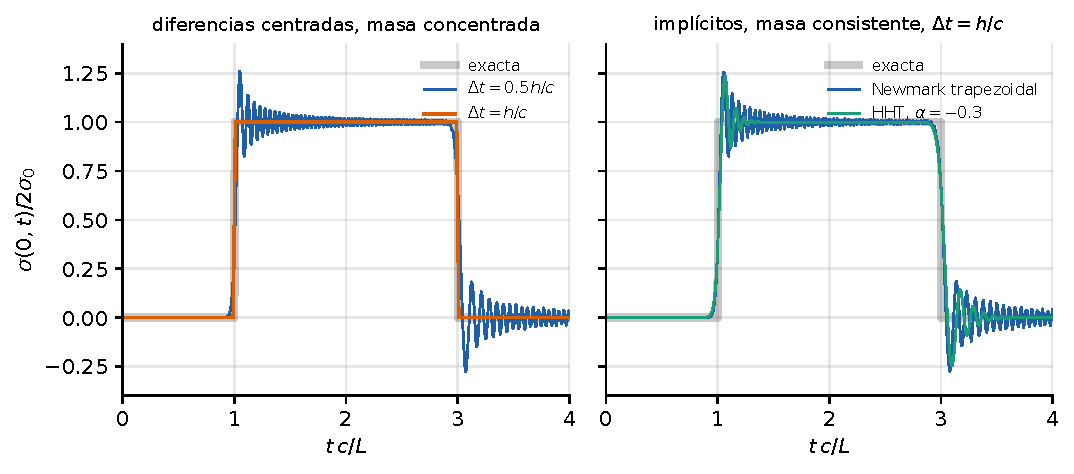
\includegraphics[width=0.9\linewidth]{../examples/onda_barra/fig_onda.pdf}
\caption{Esfuerzo en el empotramiento durante una vuelta de la onda. Izquierda: diferencias centradas con el paso límite y con la mitad. Derecha: Newmark y HHT-\ensuremath{\alpha} con el paso límite.}
\label{fig:onda_barra:onda}
\end{figure}

\begin{table}[h]
\centering
\caption{Error máximo del desplazamiento del extremo libre (relativo a $u_{\mathrm{est}}$), sobrepaso del esfuerzo en el empotramiento sobre $2\sigma_0$, y oscilación de la cola lejos de los frentes (media cuadrática entre $1.5$ y $2.8\,L/c$, relativa a $2\sigma_0$).}
\begin{tabularx}{\textwidth}{YYYYYY}
\hline
\textbf{Integrador} & \textbf{$\Delta t/(h/c)$} & \textbf{Pasos} & \textbf{Error en $u$} & \textbf{Sobrepaso de $\sigma$} & \textbf{Oscilación de la cola} \\
\hline
Diferencias centradas & 1 & 400 & $< 10^{-10}$ & $< 10^{-10}$ & $< 10^{-10}$ \\
Diferencias centradas & 0.5 & 800 & 0.017 & 0.260 & $1.5\times 10^{-2}$ \\
Newmark & 1 & 400 & 0.019 & 0.254 & $1.5\times 10^{-2}$ \\
HHT-\ensuremath{\alpha}, $\alpha = -0.3$ & 1 & 400 & 0.024 & 0.237 & $1.2\times 10^{-5}$ \\
Newmark & 4 & 100 & 0.062 & 0.280 & $8.0\times 10^{-2}$ \\
HHT-\ensuremath{\alpha}, $\alpha = -0.3$ & 4 & 100 & 0.068 & 0.262 & $1.9\times 10^{-2}$ \\
\hline
\end{tabularx}
\end{table}
\textbf{El paso límite es exacto.} Con diferencias centradas, masa concentrada y $\Delta t = h/c$, los desplazamientos nodales coinciden con la solución exacta a precisión de máquina, y el esfuerzo del primer elemento sube a $2\sigma_0$ sin sobrepasarlo. No es casualidad: la masa concentrada hace que la malla vibre con frecuencias algo menores que las reales, las diferencias centradas producen el error contrario, y con ese paso los dos se cancelan exactamente. La onda discreta avanza justo un elemento por paso.

\textbf{Un paso menor es peor.} Con la mitad del paso, el frente llega a tiempo pero arrastra oscilaciones y el esfuerzo se pasa un 26 \% del valor exacto. Es la \textbf{dispersión numérica}: las componentes de alta frecuencia del frente viajan en la malla más despacio que $c$ y se quedan atrás. Reducir el paso elimina el error temporal pero no el espacial, que ya no queda compensado.

\textbf{Los implícitos oscilan igual.} Newmark con el mismo paso da un sobrepaso parecido, del 25 \%. La disipación de HHT-\ensuremath{\alpha} casi no cambia el primer sobrepaso, pero apaga la cola de oscilaciones: su media cuadrática baja de $1.5\times 10^{-2}$ a $1.2\times 10^{-5}$. La disipación actúa sobre las frecuencias más altas, las que forman la cola; el sobrepaso del frente lo producen sobre todo frecuencias más bajas, que HHT está diseñado para respetar. Con un paso cuatro veces mayor los implícitos siguen siendo estables, pero el error en el desplazamiento crece hasta un 6 \%.

\textbf{Cuándo usar cada uno.} Para ondas e impactos, el explícito cerca de su límite es a la vez el más preciso y el más barato por paso. Los implícitos compensan cuando la respuesta la dominan los modos bajos, como la de un edificio ante un sismo (ejemplo 7): entonces el paso puede ser mucho mayor que el límite del explícito, que lo impondría el elemento más pequeño de la malla.

\section{Para seguir}

\begin{itemize}
  \item Refinar la malla a 200 elementos manteniendo el mismo $\Delta t$. ¿Qué le pasa al esquema explícito?
  \item Repetir el caso de Newmark con masa concentrada (\texttt{lumping=\textquotedbl{}lumped\textquotedbl{}}). ¿Mejora o empeora el sobrepaso?
  \item Sustituir el escalón por un pulso suave, por ejemplo medio seno de duración $20\,h/c$. ¿Qué queda de la dispersión?
\end{itemize}

\textbf{Referencias.} K.-J. Bathe, \textit{Finite Element Procedures}, 2.ª ed., 2014, cap. 9. T. J. R. Hughes, \textit{The Finite Element Method}, Dover, 2000, cap. 9. T. Belytschko, W. K. Liu y B. Moran, \textit{Nonlinear Finite Elements for Continua and Structures}, 2.ª ed., Wiley, 2014, cap. 6. H. M. Hilber, T. J. R. Hughes y R. L. Taylor, \textquotedbl{}Improved numerical dissipation for time integration algorithms in structural dynamics\textquotedbl{}, \textit{Earthquake Engineering and Structural Dynamics} 5 (1977) 283-292.

\textbf{Archivos del ejemplo.} La carpeta \texttt{examples/\allowbreak{}onda\_\allowbreak{}barra/\allowbreak{}} contiene el script \texttt{run.py}, los resultados en \texttt{resultados.json} y la figura.


\newpage

\chapter{Muro calentado bruscamente: conducción transitoria y el método θ}
\chaptermark{Muro calentado bruscamente}
\label{cap:muro_termico}





Un muro a temperatura ambiente recibe de pronto calor por una de sus caras: un fluido caliente, un incendio, el sol después de una noche fría. El calor penetra poco a poco y la temperatura de cada punto sube suavemente, sin pasarse nunca del valor de la cara. Este ejemplo resuelve ese choque térmico con el método \ensuremath{\theta} y lo compara con la solución exacta. Enseña dos cosas que no se ven en los ejemplos estáticos: el esquema temporal más preciso no siempre es el más seguro, y un resultado numérico puede ser físicamente imposible aunque el cálculo no avise de nada.

\textbf{Qué se aprende}

\begin{itemize}
  \item Resolver un transitorio térmico con \texttt{ThetaMethodSolver} y elementos \texttt{Quad4Thermal}.
  \item Elegir el parámetro \ensuremath{\theta}: Euler implícito frente a Crank-Nicolson.
  \item Reconocer las oscilaciones de Crank-Nicolson y la violación del principio del máximo.
  \item Elegir entre capacidad concentrada y consistente.
\end{itemize}

\section{Planteamiento}

Un muro de concreto de 20 cm de espesor, con conductividad $k =$ 1.4 W/(m\ensuremath{\cdot}K), densidad 2400 kg/m\ensuremath{^{3}} y calor específico 900 J/(kg\ensuremath{\cdot}K), está a $T_0 =$ 20 \ensuremath{^{\circ}}C. En $t = 0$ su cara interior pasa bruscamente a $T_s =$ 80 \ensuremath{^{\circ}}C; la exterior no intercambia calor (adiabática). El muro se modela como una franja de 40 elementos \texttt{Quad4Thermal} de $h =$ 5 mm: los bordes sin condición son adiabáticos, así que la franja representa cualquier porción del muro.

La difusividad es $\alpha = k/(\rho c) =$ $6.48\times 10^{-7}$ m\ensuremath{^{2}}/s. El tiempo característico del muro entero es $L^2/\alpha =$ 17.1 h; el de un elemento, $h^2/\alpha =$ 38.6 s.

\section{Solución analítica}

La serie de Carslaw y Jaeger para una placa con una cara a temperatura impuesta y la otra adiabática es

\[
\frac{T - T_s}{T_0 - T_s} = \sum_{n=0}^{\infty} \frac{4}{(2n+1)\,\pi}\,\sin(\lambda_n x)\,e^{-\alpha\lambda_n^2 t},
\qquad
\lambda_n = \frac{(2n+1)\,\pi}{2L} .
\]

Además, la ecuación del calor cumple el \textbf{principio del máximo}: sin fuentes internas, la temperatura de cualquier punto queda siempre entre la mínima y la máxima de los datos, aquí entre 20 y 80 \ensuremath{^{\circ}}C. Un valor fuera de ese intervalo no es impreciso: es imposible.

\section{Modelo en Solidum}

El muro y la temperatura impuesta:

\begin{lstlisting}[language=Python]
def muro():
    """Franja de ``N`` elementos ``Quad4Thermal`` a lo ancho del muro; los
    bordes sin condición son adiabáticos. Temperatura ``T_s`` en ``x = 0``."""
    dom = Domain()
    concreto = ThermalConduction(k=K, c=CP, density=RHO)
    nodos = {}
    for j in range(2):
        for i in range(N + 1):
            nodos[(i, j)] = dom.add_node(len(nodos) + 1, [i * H, j * H])
    for i in range(N):
        dom.add_element(Quad4Thermal(i + 1, [nodos[(i, 0)], nodos[(i + 1, 0)],
                                             nodos[(i + 1, 1)], nodos[(i, 1)]], concreto))
    for j in range(2):
        nodos[(0, j)].fix_dof("T", TS)
    dom.generate_equation_numbers(verbose=False)
    return dom, nodos

\end{lstlisting}

La integración en el tiempo, con el esquema y la forma de la capacidad como parámetros:

\begin{lstlisting}[language=Python]
def integrar(theta: float, dt: float, t_fin: float, capacidad: str = "lumped"):
    """Temperatura en la línea ``y = 0`` en todos los instantes."""
    dom, nodos = muro()
    solver = ThetaMethodSolver(Assembler(dom), dt=dt, n_steps=int(round(t_fin / dt)),
                               T_initial=T0, theta=theta, lumping=capacidad)
    resultado = solver.solve()
    filas = [nodos[(i, 0)].dofs["T"] for i in range(N + 1)]
    x = np.array([nodos[(i, 0)].coordinates[0] for i in range(N + 1)])
    return np.asarray(resultado.t_history), np.asarray(resultado.T_history)[filas], x

\end{lstlisting}

La condición inicial, 20 \ensuremath{^{\circ}}C, contradice la temperatura impuesta en la cara. Solidum lo avisa y lo acepta: es un choque térmico, una discontinuidad en $t = 0$ que el modelo puede representar.

\textbf{El método \ensuremath{\theta}.} Con la capacidad $\mathbf C$ y la conductividad $\mathbf K$ de la malla, cada paso resuelve

\[
\frac{\mathbf C}{\Delta t}\left(\mathbf T_{n+1} - \mathbf T_n\right) + \mathbf K\left[\theta\,\mathbf T_{n+1} + (1-\theta)\,\mathbf T_n\right] = \mathbf F .
\]

Con $\theta = 1$ es \textbf{Euler implícito}: de primer orden, pero L-estable, es decir, amortigua por completo en cada paso los modos de temperatura más rápidos. Con $\theta = 1/2$ es \textbf{Crank-Nicolson}: de segundo orden, pero no L-estable; esos modos rápidos no se amortiguan, cambian de signo en cada paso. El valor por omisión de Solidum es $\theta = 1$.

\section{Resultados}

\begin{figure}[H]
\centering
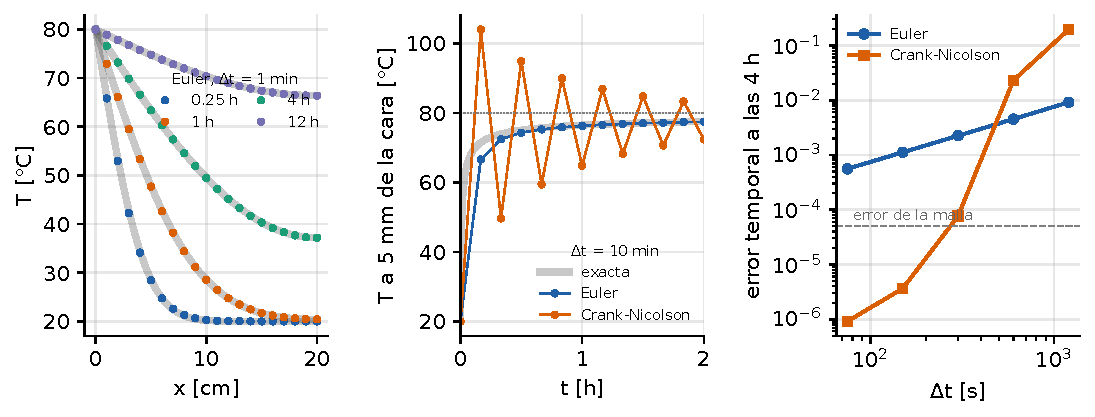
\includegraphics[width=0.9\linewidth]{../examples/muro_termico/fig_muro.pdf}
\caption{Izquierda: perfiles de temperatura a 0.25, 1, 4 y 12 h con Euler implícito y \ensuremath{\Delta}t = 1 min, sobre la solución exacta (gris). Centro: temperatura a 5 mm de la cara con \ensuremath{\Delta}t = 10 min. Derecha: error temporal a las 4 h frente al paso, y error de la malla.}
\label{fig:muro_termico:muro}
\end{figure}

\begin{table}[h]
\centering
\caption{Error temporal a las 4 h (máximo a lo ancho del muro, relativo a $T_s - T_0$), frente a una solución con $\Delta t = 1$ s en la misma malla.}
\begin{tabularx}{\textwidth}{YYY}
\hline
\textbf{$\Delta t$} & \textbf{Euler implícito} & \textbf{Crank-Nicolson} \\
\hline
20 min & $9.2\times 10^{-3}$ & $2.0\times 10^{-1}$ \\
10 min & $4.5\times 10^{-3}$ & $2.3\times 10^{-2}$ \\
5 min & $2.2\times 10^{-3}$ & $7.6\times 10^{-5}$ \\
2.5 min & $1.1\times 10^{-3}$ & $3.6\times 10^{-6}$ \\
1.25 min & $5.6\times 10^{-4}$ & $9.1\times 10^{-7}$ \\
\hline
\end{tabularx}
\end{table}
\textbf{Euler implícito sigue la solución exacta} a todas las horas (\hyperref[fig:muro_termico:muro]{figura~\ref*{fig:muro_termico:muro}}, izquierda), y nunca sale del intervalo físico. Su error temporal se reduce a la mitad cada vez que el paso se divide por dos: orden 1.00.

\textbf{Crank-Nicolson es mucho más preciso con pasos pequeños.} Su error baja con el cuadrado del paso, orden 2.00, y con 2.5 minutos ya es mucho menor que el error de la malla, $5\times 10^{-5}$: afinar más el paso no serviría sin afinar también la malla.

\textbf{Pero con pasos grandes oscila.} Con $\Delta t = 10$ min, el primer paso lleva el punto situado a 5 mm de la cara a 104 \ensuremath{^{\circ}}C, por encima de los 80 \ensuremath{^{\circ}}C de la cara (\hyperref[fig:muro_termico:muro]{figura~\ref*{fig:muro_termico:muro}}, centro). A partir de ahí la temperatura alterna por encima y por debajo de la solución durante horas. Es el modo rápido que el choque térmico excita y que Crank-Nicolson no amortigua. A las 4 h todavía no se ha extinguido, y con 10 y 20 minutos de paso Crank-Nicolson resulta peor que Euler implícito. Euler implícito, con el mismo paso, queda entre 20 y 80 \ensuremath{^{\circ}}C.

\begin{warnbox}{Advertencia}
Ante un cambio brusco ---un choque térmico, una temperatura impuesta que salta--- Crank-Nicolson necesita pasos pequeños frente al tiempo característico de un elemento, $h^2/\alpha$. En este muro, con 5 minutos (8 veces $h^2/\alpha$) todavía llega a 92.7 \ensuremath{^{\circ}}C; con 2.5 minutos (4 veces) ya no sale del rango. Con pasos mayores produce temperaturas imposibles sin que el cálculo falle ni avise. Euler implícito es menos preciso pero nunca oscila, y por eso es el valor por omisión.
\end{warnbox}

\textbf{Capacidad concentrada o consistente.} La capacidad consistente reparte la inercia térmica entre nodos vecinos, y con pasos muy pequeños eso también viola el principio del máximo. Con $\Delta t = 1$ s, menor que $h^2/(6\alpha) =$ 6.4 s, el muro se \textbf{enfría} junto a la cara antes de calentarse: llega a 19.07 \ensuremath{^{\circ}}C, por debajo de su temperatura inicial. Con $\Delta t = 8$ s el efecto desaparece, y con la capacidad concentrada no aparece con ningún paso. Es la razón de que la concentrada sea el valor por omisión.

\section{Para seguir}

\begin{itemize}
  \item Probar \ensuremath{\theta} = 2/3 (Galerkin). ¿Oscila con $\Delta t = 10$ min?
  \item Integrar con el esquema explícito, \ensuremath{\theta} = 0, y $\Delta t = 30$ s. Su límite de estabilidad con capacidad concentrada es $h^2/(2\alpha)$.
  \item Imponer en la cara un ciclo diario de temperatura con el argumento \texttt{dirichlet\_func} del solver, y medir hasta qué profundidad llega la oscilación.
\end{itemize}

\textbf{Referencias.} H. S. Carslaw y J. C. Jaeger, \textit{Conduction of Heat in Solids}, 2.ª ed., Oxford, 1959, §3.3. T. J. R. Hughes, \textit{The Finite Element Method}, Dover, 2000, cap. 8.

\textbf{Archivos del ejemplo.} La carpeta \texttt{examples/\allowbreak{}muro\_\allowbreak{}termico/\allowbreak{}} contiene el script \texttt{run.py}, los resultados en \texttt{resultados.json} y la figura.


\newpage

\chapter{Lámina ortótropa fuera de ejes: acoplamiento tracción-cortante}
\chaptermark{Lámina ortótropa fuera de ejes}
\label{cap:lamina_ortotropa}





Las fibras de un material compuesto dan mucha rigidez en su dirección y poca en las demás. Cuando la carga no sigue las fibras pasan dos cosas: la rigidez cae mucho más de lo que sugiere el ángulo, y una tracción pura distorsiona la pieza, un acoplamiento que ningún material isótropo tiene. Este ejemplo mide los dos efectos en una lámina de carbono-epoxi y los compara con la teoría clásica de láminas. Después muestra una consecuencia práctica: en el ensayo de tracción, las mordazas impiden esa distorsión y alteran el módulo que se mide.

\textbf{Qué se aprende}

\begin{itemize}
  \item Definir un material ortótropo con \texttt{Orthotropic2D} y orientar sus fibras con \texttt{theta}.
  \item Calcular las constantes aparentes de una lámina con las fibras a un ángulo cualquiera.
  \item Reconocer el acoplamiento tracción-cortante.
  \item Por qué la probeta de un ensayo fuera de ejes debe ser larga.
\end{itemize}

\section{Planteamiento}

Una lámina unidireccional de carbono-epoxi tiene $E_1 =$ 181 GPa en la dirección de las fibras (eje 1), $E_2 =$ 10.3 GPa en la transversal (eje 2), $G_{12} =$ 7.17 GPa y $\nu_{12} =$ 0.28, valores típicos de un T300/5208. Es delgada, así que trabaja en esfuerzo plano. De ella se corta una tira de ancho $w =$ 20 mm con las fibras a un ángulo $\theta$ del eje $x$, que es el eje de carga.

El caso se resuelve dos veces:

\begin{enumerate}
  \item \textbf{Tira libre.} Se tracciona con $\sigma_x =$ 10 MPa aplicada como tracción en el borde derecho. El borde izquierdo sólo tiene impedido $u_x$ (y $u_y$ en una esquina), así que la tira puede estrecharse y distorsionarse sin restricción.
  \item \textbf{Tira con mordazas.} Los dos extremos están sujetos: $u_y = 0$, y $u_x$ uniforme, nulo en un extremo y $\delta$ en el otro. Es lo que hacen las mordazas rígidas de una máquina de ensayos.
\end{enumerate}

\section{Solución analítica}

En los ejes del material la flexibilidad de esfuerzo plano es diagonal por bloques, sin acoplamiento entre alargamientos y distorsión:

\[
\mathbf S = \begin{bmatrix} 1/E_1 & -\nu_{12}/E_1 & 0 \\ -\nu_{12}/E_1 & 1/E_2 & 0 \\ 0 & 0 & 1/G_{12} \end{bmatrix},
\qquad
\frac{\nu_{21}}{E_2} = \frac{\nu_{12}}{E_1} .
\]

La segunda igualdad es la reciprocidad de Maxwell-Betti ($\mathbf S$ es simétrica). Da $\nu_{21} = \nu_{12}E_2/E_1 =$ 0.0159: con la carga transversal a las fibras, la lámina casi no se estrecha.

En los ejes de carga, la flexibilidad es $\bar{\mathbf S} = \mathbf T^{-1}\,\mathbf S\,\mathbf T^{-\top}$, con $\mathbf T$ la matriz que pasa las deformaciones de ingeniería de los ejes $x, y$ a los ejes $1, 2$. Una tracción $\sigma_x$ sola produce $\varepsilon_x = \bar S_{11}\sigma_x$, $\varepsilon_y = \bar S_{12}\sigma_x$ y $\gamma_{xy} = \bar S_{16}\sigma_x$. De ahí salen las tres constantes aparentes de la lámina:

\[
E_x = \frac{1}{\bar S_{11}}, \qquad
\nu_{xy} = -\frac{\bar S_{12}}{\bar S_{11}}, \qquad
\eta_{xy,x} = \frac{\gamma_{xy}}{\varepsilon_x} = \frac{\bar S_{16}}{\bar S_{11}} .
\]

El \textbf{coeficiente de influencia mutua} $\eta_{xy,x}$ mide el acoplamiento: la distorsión que produce una tracción, por unidad de alargamiento. Es nulo con las fibras a 0\ensuremath{^{\circ}} o a 90\ensuremath{^{\circ}} y en cualquier material isótropo. Con la tira libre el estado es uniforme, así que el cálculo debe reproducir estas fórmulas sin error de discretización.

\section{Modelo en Solidum}

La tira, con el material orientado por \texttt{theta} en grados:

\begin{lstlisting}[language=Python]
def tira(theta: float, L: float, nx: int, ny: int):
    """Tira ``L × W`` de ``nx × ny`` elementos ``Quad8`` con las fibras a
    ``theta`` grados del eje ``x``."""
    dom = Domain()
    lamina = Orthotropic2D(E1=E1, E2=E2, G12=G12, nu12=NU12, theta=theta)
    nodos = {}
    for j in range(2 * ny + 1):
        for i in range(2 * nx + 1):
            if i % 2 and j % 2:
                continue                       # centro: no es nodo del Quad8
            nodos[(i, j)] = dom.add_node(len(nodos) + 1, [L * i / (2 * nx), W * j / (2 * ny)])
    elementos = []
    for j in range(ny):
        for i in range(nx):
            a, b = 2 * i, 2 * j
            conectividad = [nodos[(a, b)], nodos[(a + 2, b)], nodos[(a + 2, b + 2)], nodos[(a, b + 2)],
                            nodos[(a + 1, b)], nodos[(a + 2, b + 1)], nodos[(a + 1, b + 2)], nodos[(a, b + 1)]]
            el = Quad8(len(dom.elements) + 1, conectividad, lamina)
            dom.add_element(el)
            elementos.append((el, i, j))
    return dom, nodos, elementos

\end{lstlisting}

La tracción libre. \texttt{compute\_\allowbreak{}edge\_\allowbreak{}traction} convierte la tracción del borde en fuerzas nodales equivalentes:

\begin{lstlisting}[language=Python]
def traccion_libre(theta: float, L: float = 2 * W, nx: int = 4, ny: int = 2) -> dict:
    """Tracción ``SIGMA`` en el borde derecho; el izquierdo sólo impide ``u_x``
    (y ``u_y`` en una esquina), así que la tira puede estrecharse y
    distorsionarse libremente: el estado es uniforme."""
    dom, nodos, elementos = tira(theta, L, nx, ny)
    for (i, j), nodo in nodos.items():
        if i == 0:
            nodo.fix_dof("ux", 0.0)
    nodos[(0, 0)].fix_dof("uy", 0.0)
    dom.generate_equation_numbers(verbose=False)
    F = np.zeros(dom.total_dofs)
    for el, i, j in elementos:
        if i == nx - 1:                       # arista derecha del Quad8: índice 1
            f = el.compute_edge_traction(1, np.array([SIGMA, 0.0]))
            F[el.get_global_dof_indices()] += f
    U = LinearSolver(Assembler(dom)).solve(F)

    def u(i, j, d):
        return U[nodos[(i, j)].dofs[d]]
    eps_x = u(2 * nx, 0, "ux") / L
    eps_y = u(0, 2 * ny, "uy") / W
    gamma = u(2 * nx, 0, "uy") / L            # u_x = 0 en x = 0: gamma = du_y/dx
    return {"E": SIGMA / eps_x, "nu": -eps_y / eps_x, "eta": gamma / eps_x,
            "deformada": _deformada(nodos, U, nx, ny)}

\end{lstlisting}

Las mordazas. Se impone el desplazamiento $\delta$ y la fuerza $P$ es la suma de las fuerzas internas en los nodos del extremo derecho. El módulo aparente es el que calcularía el laboratorio, $E_{\mathrm{ap}} = (P/w)/(\delta/L)$:

\begin{lstlisting}[language=Python]
def traccion_mordazas(theta: float, esbeltez: float, nx_por_w: int = 16, ny: int = 16) -> dict:
    """Mordazas rígidas: en los dos extremos ``u_y = 0`` y ``u_x`` uniforme
    (0 y δ). El módulo aparente es la fuerza de reacción entre ``w·δ/L``."""
    L = esbeltez * W
    nx = int(nx_por_w * esbeltez)
    dom, nodos, _ = tira(theta, L, nx, ny)
    delta = 1.0e-4 * L
    derecha = []
    for (i, j), nodo in nodos.items():
        if i == 0:
            nodo.fix_dof("ux", 0.0)
            nodo.fix_dof("uy", 0.0)
        elif i == 2 * nx:
            nodo.fix_dof("ux", delta)
            nodo.fix_dof("uy", 0.0)
            derecha.append(nodo)
    dom.generate_equation_numbers(verbose=False)
    asm = Assembler(dom)
    U = LinearSolver(asm).solve(np.zeros(dom.total_dofs))
    _, F_int = asm.assemble_non_linear_system(U)
    P = sum(F_int[nodo.dofs["ux"]] for nodo in derecha)
    return {"E": (P / W) / (delta / L), "deformada": _deformada(nodos, U, nx, ny)}

\end{lstlisting}

La tira libre usa 4 \ensuremath{\times} 2 elementos \texttt{Quad8}, porque el estado es uniforme. La tira con mordazas usa 16 elementos por ancho y se repite con 8 para comprobar la convergencia.

\section{Resultados}

\begin{figure}[H]
\centering
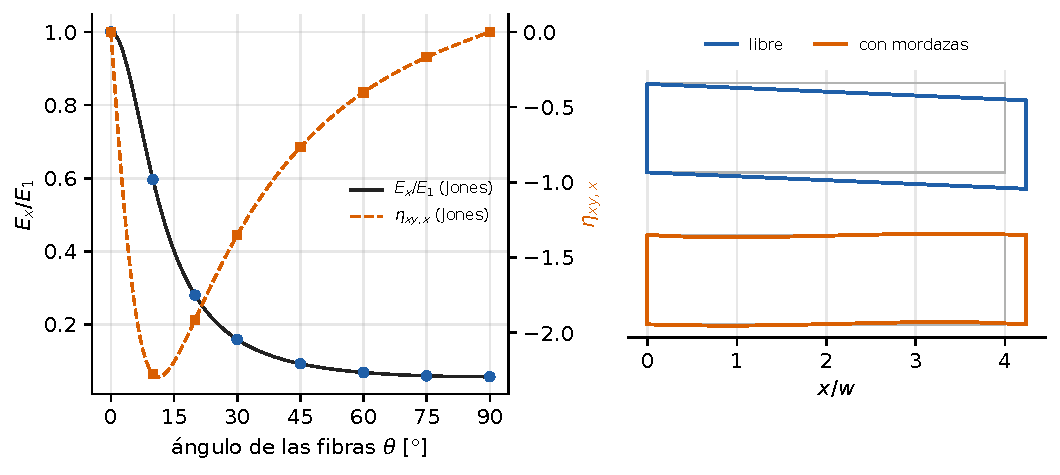
\includegraphics[width=0.9\linewidth]{../examples/lamina_ortotropa/fig_lamina.pdf}
\caption{Izquierda: módulo aparente y coeficiente de influencia mutua frente al ángulo de las fibras; curvas de la teoría de láminas y puntos de Solidum. Derecha: tira de longitud $4w$ con las fibras a 45\ensuremath{^{\circ}}, libre y con mordazas; las dos deformadas amplificadas hasta el mismo alargamiento.}
\label{fig:lamina_ortotropa:lamina}
\end{figure}

\begin{table}[h]
\centering
\caption{Constantes aparentes de la tira libre calculadas con Solidum. Todas coinciden con la teoría de láminas con una diferencia menor que $10^{-9}$.}
\begin{tabularx}{\textwidth}{YYYY}
\hline
\textbf{$\theta$} & \textbf{$E_x$ [GPa]} & \textbf{$\nu_{xy}$} & \textbf{$\eta_{xy,x}$} \\
\hline
0\ensuremath{^{\circ}} & 181.0 & 0.280 & 0 \\
10\ensuremath{^{\circ}} & 107.8 & 0.273 & $-2.274$ \\
20\ensuremath{^{\circ}} & 50.7 & 0.255 & $-1.913$ \\
30\ensuremath{^{\circ}} & 28.8 & 0.227 & $-1.351$ \\
45\ensuremath{^{\circ}} & 16.7 & 0.167 & $-0.766$ \\
60\ensuremath{^{\circ}} & 12.4 & 0.098 & $-0.402$ \\
75\ensuremath{^{\circ}} & 10.7 & 0.039 & $-0.167$ \\
90\ensuremath{^{\circ}} & 10.3 & 0.016 & 0 \\
\hline
\end{tabularx}
\end{table}
\textbf{La tira libre es exacta.} Con el estado uniforme, los \texttt{Quad8} reproducen la teoría de láminas a precisión de máquina en los ocho ángulos (\hyperref[fig:lamina_ortotropa:lamina]{figura~\ref*{fig:lamina_ortotropa:lamina}}, izquierda). A 90\ensuremath{^{\circ}} el Poisson aparente es $\nu_{21}$, la reciprocidad en acción.

\textbf{La rigidez cae deprisa.} Basta girar las fibras 10\ensuremath{^{\circ}} para que $E_x$ baje de 181 a 108 GPa. A 45\ensuremath{^{\circ}} queda en 16.7 GPa, el 9.2 \% de $E_1$, cuando el promedio de $E_1$ y $E_2$ sugeriría cerca de la mitad. La causa es el cortante: fuera de ejes, buena parte del alargamiento viene de distorsionar la matriz de resina, y $G_{12}$ es el menor de los tres módulos.

\textbf{Una tracción produce distorsión.} A 45\ensuremath{^{\circ}}, cada unidad de alargamiento viene acompañada de $-0.77$ unidades de distorsión angular, y a 10\ensuremath{^{\circ}} el acoplamiento pasa de 2. El signo tiene una lectura sencilla. Con las fibras a +45\ensuremath{^{\circ}}, la tira se alarga menos en la dirección de las fibras, que es rígida, que en la perpendicular; esa diferencia es precisamente $\gamma_{xy}$, que resulta negativa. La tira se convierte en un paralelogramo (\hyperref[fig:lamina_ortotropa:lamina]{figura~\ref*{fig:lamina_ortotropa:lamina}}, derecha).

\begin{warnbox}{Advertencia}
En Solidum, \texttt{nu12} es $-\varepsilon_2/\varepsilon_1$ con la carga en la dirección 1, la de las fibras. Algunas fuentes llaman $\nu_{12}$ al cociente contrario, que aquí vale 0.016. Si se copia ese valor, el cálculo no falla y el material resultante es otro: su contracción transversal es $E_1/E_2$ veces menor que la real.
\end{warnbox}

\textbf{Las mordazas impiden la distorsión.} Con los extremos sujetos, la tira no puede convertirse en paralelogramo. Junto a las mordazas no puede distorsionarse; lejos de ellas sí, y para hacer compatibles las dos zonas se flexiona en su plano: se deforma en S (\hyperref[fig:lamina_ortotropa:lamina]{figura~\ref*{fig:lamina_ortotropa:lamina}}, derecha). Impedir una deformación rigidiza, así que el módulo aparente crece.

\begin{table}[h]
\centering
\caption{Módulo aparente con mordazas, relativo al de la tira libre $E_x$. La última fila es la cota superior $\bar Q_{11}/E_x$.}
\begin{tabularx}{\textwidth}{YYY}
\hline
\textbf{$L/w$} & \textbf{$\theta = 30°$} & \textbf{$\theta = 45°$} \\
\hline
2 & 1.61 & 1.19 \\
4 & 1.15 & 1.05 \\
8 & 1.04 & 1.01 \\
Cota superior & 3.80 & 3.39 \\
\hline
\end{tabularx}
\end{table}
Este resultado es numérico, sin solución cerrada. Pasar de 8 a 16 elementos por ancho cambia el módulo aparente como mucho en $10^{-2}$ (30\ensuremath{^{\circ}}, $L/w = 2$), así que las cifras de la tabla son fiables al 1 \%. Además, los teoremas de energía lo acotan por los dos lados:

\begin{itemize}
  \item \textbf{Por abajo, $E_x$.} El esfuerzo uniforme de la tira libre está en equilibrio y es compatible con las mordazas. El teorema de la mínima energía complementaria da $E_{\mathrm{ap}} \ge E_x$.
  \item \textbf{Por arriba, $\bar Q_{11}$.} El desplazamiento uniforme $\varepsilon_x = \delta/L$, $\varepsilon_y = \gamma_{xy} = 0$ cumple las condiciones de las mordazas. El teorema de la mínima energía potencial da $E_{\mathrm{ap}} \le \bar Q_{11}$, con $\bar{\mathbf Q} = \bar{\mathbf S}^{-1}$ la rigidez de la lámina en ejes de carga. Es el módulo de una tira infinitamente corta, sujeta en toda su longitud.
\end{itemize}

Los seis casos caen dentro de las cotas. Cuanto más corta es la tira, más rígida resulta: con $L/w = 2$ el módulo medido a 45\ensuremath{^{\circ}} excede a $E_x$ en un 19 \%, y a 30\ensuremath{^{\circ}} en un 61 \%. A 30\ensuremath{^{\circ}} el efecto es mayor porque el acoplamiento es mayor, $\eta_{xy,x} =$ $-1.35$ frente a $-0.77$: hay más distorsión que impedir.

\begin{warnbox}{Advertencia}
Un ensayo de tracción fuera de ejes con una probeta corta sobreestima el módulo y no avisa: la curva fuerza-desplazamiento sale perfectamente lineal. Aun con $L/w = 8$, el error es del 1.2 \% a 45\ensuremath{^{\circ}} y del 3.6 \% a 30\ensuremath{^{\circ}}. Por eso las probetas fuera de ejes se hacen largas y esbeltas.
\end{warnbox}

\section{Para seguir}

\begin{itemize}
  \item Repetir la tira con mordazas a 10\ensuremath{^{\circ}}, cerca del ángulo de mayor acoplamiento. ¿Cuánto crece el módulo aparente con $L/w = 8$?
  \item Medir el alargamiento con un extensómetro virtual: la diferencia de $u_x$ entre dos puntos del centro de la tira, en vez de $\delta/L$. ¿Se recupera $E_x$?
  \item Cambiar el material por uno de vidrio-epoxi, con $E_1/E_2$ mucho menor. ¿Qué pasa con $\eta_{xy,x}$?
\end{itemize}

\textbf{Referencias.} R. M. Jones, \textit{Mechanics of Composite Materials}, 2.ª ed., Taylor \& Francis, 1999, cap. 2. N. J. Pagano y J. C. Halpin, \textquotedbl{}Influence of end constraint in the testing of anisotropic bodies\textquotedbl{}, \textit{Journal of Composite Materials} 2 (1968) 18-31.

\textbf{Archivos del ejemplo.} La carpeta \texttt{examples/\allowbreak{}lamina\_\allowbreak{}ortotropa/\allowbreak{}} contiene el script \texttt{run.py}, los resultados en \texttt{resultados.json} y la figura.


\newpage

\clearpage
\thispagestyle{empty}
\vspace*{\fill}
\begin{center}
\rule{0.4\textwidth}{0.4pt}\\[1em]
{\bfseries\color{yamlkey} Solidum FEM --- Manual de Ejemplos}\\[0.5em]
Sigla del manual: \texttt{FF-ME}\\[0.5em]
Compilado el 24 de septiembre de 2026, 08:04\\[0.5em]
Commit Git: \texttt{7c5e48f} (con cambios sin confirmar)\\[1em]
\rule{0.4\textwidth}{0.4pt}\\[2em]
\parbox{0.75\textwidth}{\small\itshape\centering
Documento generado automáticamente desde \texttt{manuals/sources/examples/} y los scripts de \texttt{examples/} mediante \texttt{python manuals/build\_example\_manual.py}. No editar directamente el PDF: cualquier corrección debe realizarse sobre el archivo fuente correspondiente y regenerar el manual.}
\end{center}
\vspace*{\fill}

\end{document}
